%KECReportFormat.tex
%%%%%%%%%%%%%%%%%%%%%%%%%%%%%%%%%%%%%%%%%%%%%%%%%%%%%%%%%%%%%%%%%%%%%%%%%%%
%DO NOT MAKE CHANGES IN THIS FILE

\documentclass[12pt, a4paper]{report}
\usepackage[left = 1.5in, right = 1in, top = 1in, bottom = 1in]{geometry}%for margin
\usepackage{amsfonts, amsmath, amssymb} %for mathematical equations
\usepackage{graphicx} %for images


\usepackage{times} %font Times New Roman Font
\usepackage{float} %required if you use H(strictly here) position for floats
\usepackage[skip = 8pt,tableposition=top, figureposition=bottom]{caption}%adjust spacing of captions and specify where captions are
\usepackage{hyperref} % for easy Navigation in document, also puts links in TOC, LOF, LOT...
\usepackage{setspace} %to change line spacing in some portion \singlespacing \onehalfspacing \doublespacing
\usepackage{acro} %for List of Abbrreviation and Symbol
\acsetup{first-style = short} % set to display only short form on the command \ac{}

%packages required for complex tables
\usepackage{bigstrut} 
\usepackage{multirow}
%package for greek letters

\renewcommand{\contentsname}{Table of Contents} %Change TOC Heading ... default is "Contents" 

\parindent 0pt	%removes the indent in paragraph
\setlength{\parskip}{18pt}	%for paragraph spacing
\renewcommand{\baselinestretch}{1.5}   %Line Spacing = 1.5 line-spaces

%to reduce spacing in sections
\usepackage{titlesec}
\titlespacing*{\section}{0pt}{0pt}{0pt} %left, top, bottom spacings
\titlespacing*{\subsection}{0pt}{0pt}{0pt}
\titlespacing*{\subsubsection}{0pt}{0pt}{0pt}
\titlespacing*{\paragraph}{0pt}{0pt}{0pt}
\titlespacing*{\subparagraph}{0pt}{0pt}{0pt}

%adjust fontsizes\ of sections
\titleformat*{\section}{\fontsize{14pt}{18pt}\bfseries}
\titleformat*{\subsection}{\fontsize{13pt}{18pt}\bfseries}
\titleformat*{\subsubsection}{\fontsize{12pt}{18pt}\bfseries}
\titleformat*{\paragraph}{\fontsize{12pt}{18pt}\bfseries}
\titleformat*{\subparagraph}{\fontsize{12pt}{18pt}\bfseries}

%to reduce separation between points in list
\usepackage{enumitem}
\setlist[enumerate]{nosep} % no separation between items in enumerate
\setlist[itemize]{nosep} % no separation between items in itemize
%use \vspace{-18pt} before list to reduce paragraph spacing between list and preceeding paragraph.

%Changes for Chapter Heading Spacing and formats for numbered chapters
\makeatletter
\def\@makechapterhead#1{%
  %\vspace*{50pt}%
  {  \MakeUppercase{\ifnum \c@secnumdepth >\m@ne
        \fontsize{16pt}{1}\bfseries \@chapapp \space \thechapter\vspace{5pt}\\
    \fi
    \interlinepenalty\@M
     \bfseries #1}\par\nobreak
    %\vskip 0pt
  }}
\makeatother

%%%%%%%%%%%%%%%%%%%%%%%%%%%%%%%%%%%%%%%%%%%%%%%%%%%%%%%%%%%
%to adjust Heading spacings and fonts For unnumbered chapters, TOC, LOF ...
\makeatletter
% Redefine the \chapter* header macro to remove vertical space
\def\@makeschapterhead#1{%
  %\vspace*{50\p@}% Remove the vertical space
  {\newpage \parindent \z@ \raggedright
    \normalfont
    \interlinepenalty\@M
    \center \fontsize{16pt}{1} \bfseries \MakeUppercase{#1}\par\nobreak
    %\vskip 18\p@ % adjust space after heading 18pt
  }}
\makeatother 
%%%%%%%%%%%%%%%%%%%%%%%%%%%%%%%%%%%%%%%%%%%%%%%%%%%%%%%%%%%

%%%%%%%%%%%%%%%%%%%%%%%%%%%%%%%%%%%%%%%%%%%%%%%%%%%%%%%%%%%%%%%%%%%%%%%%%%%
% newcommand for generating Cover Page
\newcommand{\KECcoverpage}
{
\begin{titlepage}
\begin{center}
\Large{\textbf{KANTIPUR ENGINEERING COLLEGE}}\\
\large{\textbf{(Affiliated to Tribhuvan University)}}\\
\large{\textbf{Dhapakhel, Lalitpur}}\\
\vfill	%vertically fill the space 
\begin{figure}[h] % h: put logo "here"
\begin{center}

\includegraphics[width=25mm, height = 25mm]{images/logo.png}
\end{center}
\end{figure}

\large{\textbf{[Subject Code: \subCode]}}\\ %Change This Line
\large{\textbf{A \MakeUppercase{\project} \MakeUppercase{\doc} ON}}\\ %Change This Line
\Large{\textbf{\MakeUppercase{\projectTitle}}}\\

\vfill	%vertically fill the space 
\large{\textbf{Submitted by:}}\\
\large{\textbf{\submittedBy}}\\
\vfill	%vertically fill the space 
\textbf{A \MakeUppercase{\project} SUBMITTED IN PARTIAL FULFILLMENT OF THE REQUIREMENT FOR THE DEGREE OF \MakeUppercase{\degree}}\\

\vfill	%vertically fill the space 
\large{\textbf{Submitted to:}}\\
\large{\textbf{\submittedTo}}\\
\vfill
\large{\textbf{\defMonth, \defYear}}
\pagebreak
\end{center}
\end{titlepage}
}
%%%%%%%%%%%%%%%%%%%%%%%%%%%%%%%%%%%%%%%%%%%%%%%%%%%%%%%%%%%%%%%%%%%%%%%
% newcommand for generating Cover Page
%Title Page
\newcommand{\KECtitlepage}
{
\begin{titlepage}
\begin{center}
\Large{\textbf{\MakeUppercase{\projectTitle}}}\\

\vfill	%vertically fill the space 

\large{\textbf{Submitted by:}}\\
\large{\textbf{\submittedBy}}\\

\if{\ne{\supervisor}{none}} \\ Displays Supervisor name only if it is not "none"
	\vfill	%vertically fill the space 
	\large{\textbf{Supervised by:}}\\
	\large{\textbf{\supervisor}}\\
	\large{\textbf{\degSup}}\\
\fi
\vfill	%vertically fill the space 
\textbf{A \MakeUppercase{\project} SUBMITTED IN PARTIAL FULFILLMENT OF THE REQUIREMENT FOR THE DEGREE OF \MakeUppercase{\degree}}\\

\vfill	%vertically fill the space 
\large{\textbf{Submitted to:}}\\
\large{\textbf{\submittedTo}}\\
\large{\textbf{Kantipur Engineering College}}\\
\large{\textbf{Dhapakhel, Lalitpur}}\\

\vfill
\large{\textbf{\defMonth, \defYear}}
\thispagestyle{empty}\\ %to remove page number
\pagebreak
\end{center}
\end{titlepage}
}
%%%%%%%%%%%%%%%%%%%%%%%%%%%%%%%%%%%%%%%%%%%%%%%%%%%%%%%%%%%%%%%%%%%%%%
%command for copyright page
\newcommand{\KECcopyright}
{
\chapter*{Copyright}%Required only for Final Defense of Major Project
\addcontentsline{toc}{chapter}{Copyright}
The author has agreed that the library, Kantipur Engineering Collage, may make this report freely available for inspection. Moreover the author has agreed that permission for extensive copying of this report for scholarly purpose may be granted by the supervisor(s), who supervised the project work recorded herein or, in their absence, by the Head of the Department wherein this project was done. It is understood that due recognition will be given to the author of this report and to the \submittedTo, Kantipur Engineering College in any use of the material of this report. Copying or publication or other use of this report for financial gain without approval of the \submittedTo, Kantipur Engineering College and author’s written permission is prohibited.\par Request for permission to copy or to make any other use of the material in this report in whole or in part should be addressed to:

Head\\
\submittedTo\\
Kantipur Engineering College\\
Dhapakhel, Lalitpur\\
Nepal
}
%%%%%%%%%%%%%%%%%%%%%%%%%%%%%%%%%%%%%%%%%%%%%%%%%%%%%%%%%%%%%%%%%%%%%%
%command for Approval Letter
\newcommand{\KECapproval}
{
\chapter*{Kantipur Engineering College
\vskip -10pt}%Required only for Final Defense of Major Project
\begin{center}
\fontsize{12.8pt}{1} %size decreaced to adjust department name in single line
\textbf{
\MakeUppercase{\submittedTo}\\ %for department name
}
\vskip 10pt
\fontsize{16pt}{1}
\textbf{APPROVAL LETTER}
\end{center}
\vskip -16pt
\addcontentsline{toc}{chapter}{Approval Letter}%
The undersigned certify that they have read and recommended to the Institute of Engineering for acceptance, a project report entitled "\projectTitle " submitted by \\
\submittedBy \\
in partial fulfillment for the degree of \degree. \par
{\vspace{25pt}
..........................................\\
%Supervisor\\
\supervisor \\
\degSup\\
\vspace{25pt}\\
..........................................\\
External Examiner\\
\external\\
\degExternal\\
\vspace{25pt}\\
..........................................\\
\hod\\
Head of Department\\
\submittedTo
\vspace{10pt}\\
Date: \defMonth\space\defDay ,\space \defYear
\singlespacing\par
} %single spacing for the texts inside {}
}

%command for list of abbreviations
\newcommand{\KECloa}
{
%\chapter*{List of Abbreviations}
\addcontentsline{toc}{chapter}{List of Abbreviations}
\vskip -42pt % to reduce space due to invisivle acronym class name
{
\singlespacing
\printacronyms[include-classes=abbr, name= List of Abbreviations ]
}

}

%command for list of symbols
\newcommand{\KEClos}
{
\chapter*{List of Symbols}
\addcontentsline{toc}{chapter}{List of Symbols}
\vskip -42pt % to reduce space due to invisivle acronym class name{
{
\singlespacing
}
}

%command to adjust toc, lof, lot spacing
\newcommand{\KECadjusttocspacings}
{
\parskip 0pt % to remove paragraph spacing in TOC, LOF ...
\renewcommand{\baselinestretch}{0.1} % to adjust line spacing in toc
\newcommand*{\noaddvspace}{\renewcommand*{\addvspace}[1]{}}
\addtocontents{lof}{\protect\noaddvspace} %remove extra vertical space in LOF
\addtocontents{lot}{\protect\noaddvspace} %remove extra vertical space in LOT
}

 %includes the file KecReportFormat.tex that include all  necessary formattings

%%%%%%%%%%%%%%%%%%%%%%%%%%%%%%%%%%%%%%%%%%%%%%%%%%%%%%%%%%%%%%%%%%%%%%%%%%%
%Define Macros for Details of your Project
\newcommand{\project}{Minor Project } %Specify "Major Project" or "Minor Project"
\newcommand{\projectTitle}{Thyroid Classification with L1 Regularization for Effective Feature Selection} %specify "Title" of Your Project
\newcommand{\doc}{Final Report} % specify the document you are preparing eg. "Proposal", "Mid-Term Report" or "Final Report"32
% Note that You have to sibmit "Final Report" for Pre-final defense as well.
\newcommand{\subCode}{CT654} %specify Subject of Your Project
\newcommand{\degree}{Bachelor in Computer Engineering} %specify your degree
\newcommand{\submittedBy}%Specify Names and Roll/Symbol Numbers of the Project Group Members
{
%Edit Member Names and Roll/Symbol No. and adjust width (\makebox[width]) if necessary 
\makebox[7cm]{Aadarsha Regmi\hfill [31051]}\\
\makebox[7cm]{Angel Tamang \hfill [31060]}\\
\makebox[7cm]{Anil Bhatta \hfill [31061]}\\
\makebox[7cm]{Manish Karki \hfill [31090]}
%\makebox[9cm]{Member Name \hfill [Roll/Symbol No.]}\\
} % Note that You must write your "Symbol Numbers"(Exam Roll Numbers) for Final Defenses

\newcommand{\submittedTo}{Department of Computer and Electronics Engineering} %specify your department
\newcommand{\hod}{Er. Rabindra Khati\\Associate Professor} %specify Head ot the department
\newcommand{\defYear}{2024} %Defense Year
\newcommand{\defMonth}{March} %Defense Month- January, February, ...
\newcommand{\defDay}{1} %specify Defense Day- 1, 2, ...

\newif\ifhassupervisor
\hassupervisortrue % to display supervisor name use command- \hassupervisortrue
 
\newcommand{\supervisor}{Er. Bishal Thapa} % Specify Name of Supervisor for Major Project
\newcommand{\degSup}{Project Coordinator\\ Department of Computer and Electronics Engineering} %Specify Designation of Supervisor for Major Project, use multiple lines (\\) if necessary
\newcommand{\external}{External} %Specify Name of External for Major Project (Required for Black Book)
\newcommand{\degExternal}{External's Designation} %Specify Name of External for Major Project (Required for Black Book) , use multiple lines (\\) if necessary
%Second Line of Designation (if required)

%%%%%%%%%%%%%%%%%%%%%%%%%%%%%%%%%%%%%%%%%%%%%%%%%%%%%%%%%%%%%%%%%%%%%%%%%%%

%%%%%%%%%%%%%%%%%%%%%%%%%%%%%%%%%%%%%%%%%%%%%%%%%%%%%%%%%%%%%%%%%%%%%%%%%%%
%Define Abberviations and Symbols
% NOTE that Only those Abberviations and Symbols that are included in document(using command \ac{}) will be displayed in the List of Abberviations and Symbols.

%class 'abbr': for List of Abbreviations



%%%%%%%%%%%%%%%%%%%%%%%%%%%%%%%%%%%%%%%%%%%%%%%%%%%%%%%%%%%%%%%%%
% class `symbol': for List of Symbols
%\DeclareAcronym{transparencyFactor}{
%  short = \ensuremath{\alpha} ,
 % long  = Transparency Factor ,
 % sort  = Transparency Factor , % string to compare for sorting symbols... default string is the acronym name -"transparencyFactor"
  %class = symbol
%}% declares acronym named "transparencyFactor". Use \ac{UN} for short and \acl{UN} for long form.

%\DeclareAcronym{areaOfTriangle}{
 % short = \ensuremath{a} , % use \ensuremath{a} instead of $a$
 %% long  = Area of Triangle ,
 % sort  = Area of Triangle , % string to compare for sorting symbols
  %class = symbol
%}
%%%%%%%%%%%%%%%%%%%%%%%%%%%%%%%%%%%%%%%%%%%%%%%%%%%%%%%%%%%%%%%%%%%%%%%%%%%%%%%%%%%%%%%%%%%%%%%%%%%%















\usepackage{array}
%\renewcommand{\thefigure}{\thesection.\arabic{figure}}

%The Document
\begin{document}

\KECcoverpage
\KECtitlepage
\KECapproval
\pagenumbering{roman}


\chapter*{Acknowledgment}
\addcontentsline{toc}{chapter}{Acknowledgment}%to include this chapter in TOC
We are grateful to everyone who contributed to the completion of this project. Firstly, we acknowledge the invaluable guidance, support, and feedback from our teachers in the Department of Electronics and Computer Engineering. We also extend our thanks to our classmates for their constructive feedback and engaging discussions about our project. Additionally, we appreciate the guidance provided by all lecturers in our department from the project's inception to its completion. Lastly, we express special gratitude to our family and friends for their love, encouragement, and support throughout our academic journey.\\
Thank you all for your invaluable contributions to this project.\\
\makebox[10cm]{Aadarsha Regmi \hfill [31051]}\\
\makebox[10cm]{Angel Tamang\hfill [31060]}\\
\makebox[10cm]{Anil Bhatta\hfill [31061]}\\
\makebox[10cm]{Manish Karki \hfill [31090]}


\chapter*{Abstract}
\addcontentsline{toc}{chapter}{Abstract}%to include this chapter in TOC 
Thyroid disease, mainly caused by disfunctioning thyroid gland that plays a crucial role in regulating various bodily functions, has emerged as a serious health concern for many individuals as it is more common than one can imagine imbalances in thyroid hormone levels can affect metabolism, energy production and numerous organs. 
The early diagnosis of thyroid disease may benefit from the use of machine learning. The project utilizes max-voting ensembled classifier to identify thyroid conditions, namely hypothyroidism and hyperthyroidism. The dataset acquired is balanced to prevent bias by the models used, and to identify relevant features among available attributes of the data, L1 regularization was utilized which is a natural candidate in a feature selection process. L1 regularization imposes a penalty term to the loss function of a model during optimization creating a sparse features vector. Thus, irrelevant features coefficients is drived to zero encouraging effective feature selection. The classification model is reliable with high recall value observed during its evaluation on testing datas.


\par
\textbf{\textit{Keywords}} \textit{$-$Machine learning, Thyroid disease, Classification model, Decision tree, Random forest, Support Vector Machines, Multi-Layer Perceptron, Ensemble, L1 regularization, Streamlit.}

%{\par
%\begin{flushright}
%\vskip -20pt
%\setstretch{1.2}
%\submittedBy
%\end{flushright}}
















%to adjust spacings for TOC, LOF, LOT
{

%TOC, LOF and LOT
\KECadjusttocspacings % defined in KECReportFormat.tex to adjust spacings
\makeatletter
% to add vskip of 18 point which is reduced when parskip is set to 0 in \LECadjustspacings
\def\@makeschapterhead#1{%
  %\vspace*{50\p@}% Remove the vertical space
  {\newpage \parindent \z@ \raggedright
    \normalfont
    \interlinepenalty\@M
    \center \fontsize{16pt}{1} \bfseries \MakeUppercase{#1}\par\nobreak
    \vskip 18\p@ % adjust space after heading 18pt
  }}
\makeatother 



\tableofcontents % prints table of contents
\listoffigures % prints list of figures
\addcontentsline{toc}{chapter}{List Of Figures}
%\listoftables % prints list of table
\listoftables % prints list of tables
\addcontentsline{toc}{chapter}{List Of Tables}
}
%%%%%%%%%%%%%%%%%%%%%%%%%%%%%%%%%%%%%%%%%%%%%%%%%%%%%%%%%%%%%%%%%%%%%%%%%%%

%comment this chapter if you don't have List of Abbreviations
%\KECloa % defined in KECReportFormat

%comment this chapter if you don't have List of Symbols
%\KEClos % defined in KECReportFormat
%\KECapproval
%\KECcopyright

\chapter*{Abbreviations}
\addcontentsline{toc}{chapter}{Abbreviations}
\begin{tabbing}
\hspace{50mm}\=\kill
DTC \>	Decision Tree Classification\\
EDA \>	Exploratory Data Analysis\\
ML \>	Machine Learning\\
ROC \>	Receiver Operating Characteristics\\
PR \>	Precision-Recall\\
RF \> Random Forest\\
MLP \> Multi-Layer Perceptron\\
SVM \> Support Vector Machines\\
\end{tabbing}


















\newpage
\pagenumbering{arabic}

\chapter{Introduction}
\setcounter{figure}{0} % Reset the figure counter

\section{Background}\label{sec:bkgrnd}%label your section if you require to refer them somewhere else in your document.
Thyroid disease is a significant global health concern, affecting millions of people worldwide. The thyroid gland, a vital organ in our body, plays a crucial role in metabolism, growth, and development. It produces two main hormones, thyroxine (T4) and triiodothyronine (T3), which are essential for the body's metabolic processes. The production of these hormones is regulated by thyroid-stimulating hormone (TSH), which is released by the pituitary gland. An imbalance in these hormones can lead to thyroid diseases.
Thyroid diseases can be broadly classified into conditions that affect the structure of the gland, such as goiter and thyroid nodules, and those that affect the function of the gland, such as hypothyroidism, hyperthyroidism, and thyroiditis. Hypothyroidism is a condition where the thyroid gland does not produce enough thyroid hormones, leading to symptoms like fatigue, weight gain, and depression. On the other hand, hyperthyroidism is a condition where the thyroid gland produces too much thyroid hormones, leading to symptoms like rapid heart rate, weight loss, and anxiety. Thyroiditis is an inflammation of the thyroid gland, which can cause either hyperthyroidism or hypothyroidism. More serious conditions include thyroid cancer and autoimmune thyroid diseases, such as Graves' disease and Hashimoto's thyroiditis.
In the context of Nepal, thyroid disorders are prevalent, with a study showing that the prevalence of thyroid dysfunction was 17.42\% among the population of the western region of Nepal \cite{yadav2013}. However, this project will not be using a dataset specific to Nepal.

Machine learning, a subset of artificial intelligence, has shown great promise in the field of healthcare, particularly in disease diagnosis. It has the potential to improve the accuracy and speed of diagnosis. In recent years, there has been a growing interest in applying machine learning algorithms for thyroid disease classification.
\begin{figure}[h]
   
    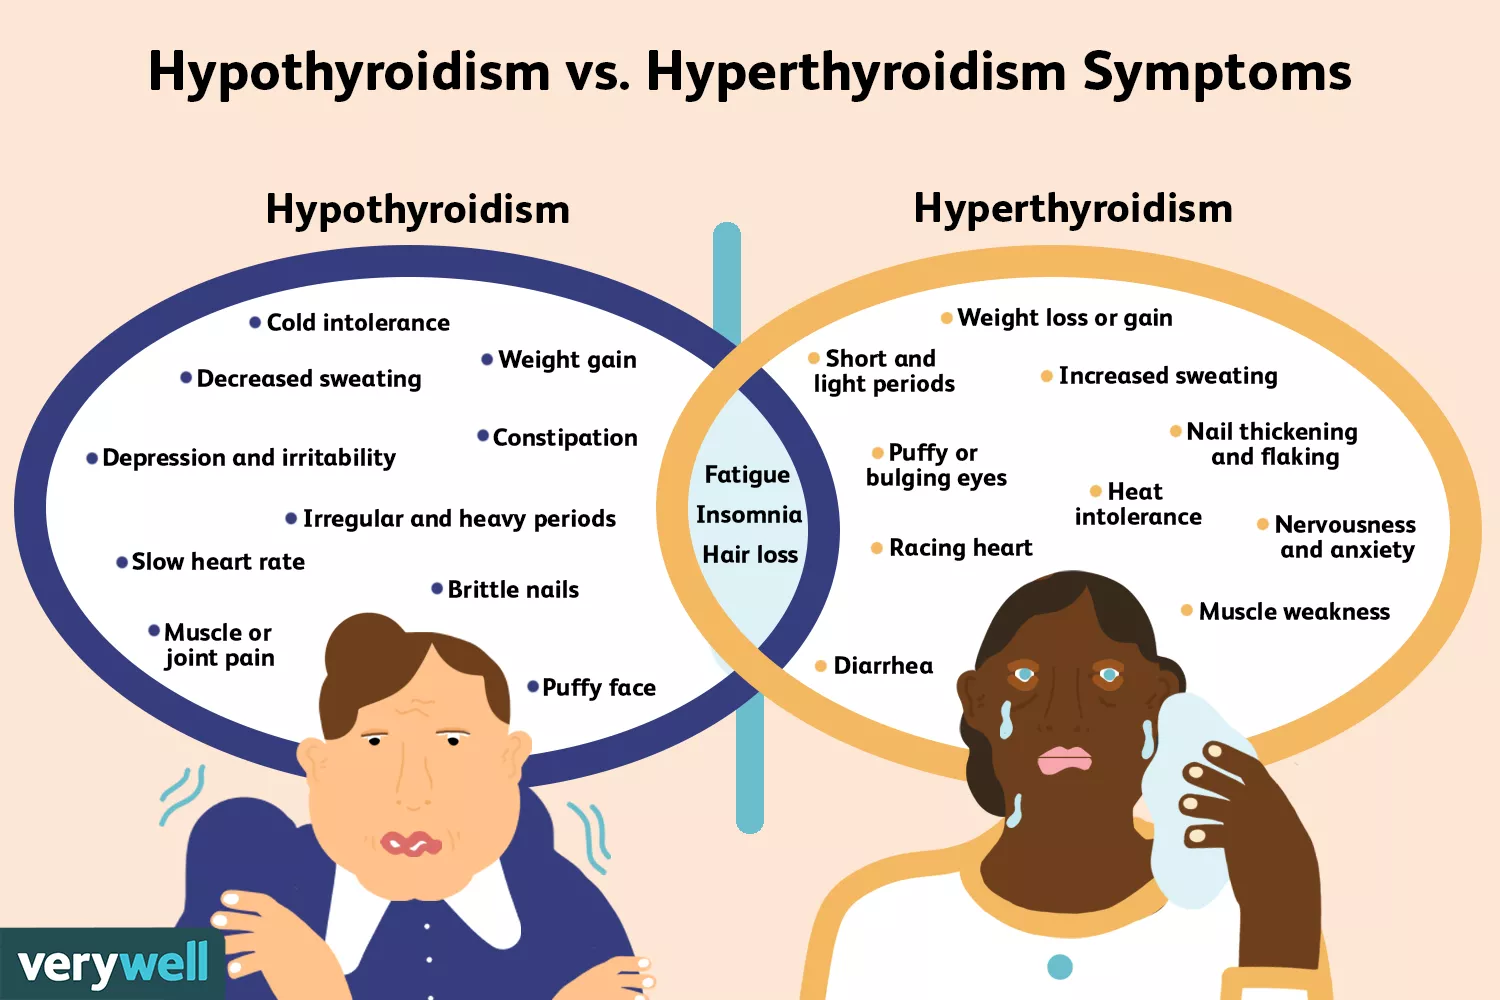
\includegraphics[scale=0.25]{thyroid.png}
    \caption{Symptoms}
    \label{fig:example}
    %\addcontentsline{toc}{subsection}{\numberline{}Example Image}
	\textit{Source:https://www.verywellhealth.com/hypothyroidism-hyperthyroidism-5180646}
    \end{figure}
      
\section{Problem Statement}
Thyroid diseases are a significant health concern due to their prevalence and potential impact on quality of life. Accurate and timely diagnosis is crucial for effective treatment and management. The interpretation of thyroid function tests can be complex due to various influencing factors such as Thyroid Stimulating Hormone(TSH), thyroxine (T4) and triiodothyronine (T3).
Machine learning algorithms, such as Decision trees, Random Forest, MLP offer a promising solution to these challenges. They have the potential to improve the accuracy and speed of diagnosis by learning from patterns in the data. However, their application in thyroid disease classification is still an emerging field and needs further research. This project aims to develop a Classification model for thyroid disease classification using a dataset that is not specific to any particular region.
\newpage
\section{Objectives}
To classify thyroid diseases, the specific objectives are as follows:
\begin{enumerate}[label=\roman*]
    \item To build classification models for thyroid disease classification.
    \item To provide a web-tool to the users for reliable thyroid testing.
\end{enumerate}

\section{Application Scope}
The application of machine learning in the classification of thyroid diseases has the potential to revolutionize the way these diseases are diagnosed and managed. The model in this project could serve as a valuable tool for healthcare professionals, aiding in the accurate and timely diagnosis of thyroid diseases. The scope of this project is broad, as the dataset used for model development is not specific to any particular region. This enhances the applicability and relevance of the project findings, potentially benefiting a wider population. The project also aims to contribute to the growing body of research on the application of machine learning in healthcare, particularly in the context of thyroid disease classification.
\section{Features}
The key features of this project include:
\begin{itemize}
\item Use of Classification algorithms for thyroid disease classification.
\item Comprehensive data analysis and preprocessing.
\item Development and rigorous evaluation of the models.
\item Performance evaluation of the developed model using appropriate metrics.
\item Comparison of the models with each other.
\item Broad applicability due to the use of a non-region-specific dataset.
\end{itemize}
\section{System Requirements}
This project needs certain hardware and software requirements in order to be developed and run. These requirements are discussed below:
%\newpage
\subsection{Development Requirements}
\begin{table}[h]
\caption{Table 1 Development Requirements}
\begin{tabular}{|c|c|}
\hline
Hardware Requirements & Software Requirements \\
\hline
Personal Computer/laptop with the specifications: & OS:windows 7 and above.\\
\begin{minipage}{8.5cm} % Adjust width as needed
     -RAM: 8GB(minimum)\\
     -Processor: CPU with four or more threads\\
     -512GB HDD or SSD(recommended)\\
     -GPU: recommended if possible\\
\end{minipage} &
\begin{minipage}{4.5cm} % Adjust width as needed

     -Python\\
     -Jupyter notebook\\
     -ML framework:\\    
        Scikit-learn, Numpy, Pandas, Matplotlib, seaborn, imblearn and so on.\\
\end{minipage}\\
\hline
\end{tabular}
\end{table}

\subsection{Deployment Requirements}
\begin{table}[h]
    \caption{Table 2 Deployment Requirements}
    
    \begin{tabular}{|c|c|}\hline
    Hardware Requirements & Software Requirements\\
    \hline
  
    Personal Computer/laptop with the specifications: &  OS: windows 7 and above.\\
	\begin{minipage}{8cm}
	
    -RAM: 8GB(minimum) \\
    -Processor: CPU with four or more threads \\    
    -Storage: 512GB HDD or SSD(recommended) \\
    -GPU: recommended if possible \\
	\end{minipage} &
	\begin{minipage}{4.5cm}
	-Visual Studio Code\\
	-Streamlit\\
	-Pickle\\
	-Python\\
	
\end{minipage}\\	    
    \hline
    \end{tabular}
\end{table}


\section{Feasibility Study}

\subsection{Economic Feasibility}
This system is economically feasible which consists of a laptop or a personal computer without any expense of other items. Nowadays, almost every house has access to the internet, so our system is economically feasible.
\subsection{Operational Feasibility}
For the operation of the system, the person doesn’t need to be an expert in using a computer.  Someone with minimum knowledge about computers and technology can also benefit from the system. There is no requirement for huge and expensive hardware.\subsection{Schedule Feasibility}
Since the development team has the capacity and basic understanding of the project, the project was completed in 7 month time period.\\\\

%(GAntt chart here)


\begin{figure}[h]
    \centering
    \includegraphics[scale=0.55]{ganttchart.png}
    \caption{Gantt Chart}
    \label{fig:my_label}
\end{figure}



\chapter{Litreature Review}

 

\section{Related Research}
According to the paper ``Thyroid function", Iodine is most important as a component of the hormones, thyroxine and 3,3,5-triiodothyronine (T3). The recommended daily iodine requirement is 150-200\(\mu\)g. Since iodine is a crucial constituent of thyroid hormones, it is not surprising that thyroid dysfunction is very common in geographical areas of iodine deficiency. However, even when this trace element is present in adequate supply, thyroid disease is present in 3-5\% of the population. Furthermore, the regulated supply of thyroid hormone to specific tissues is crucial during fetal development \cite{arthur_beckett_1999}.

Paper ``Thyroid Disease Classification Using Machine Learning Algorithms” aims to classify thyroid conditions because medical reports show serious imbalances in thyroid diseases. The data was applied to a range of machine learning algorithms (Decision Tree, SVM, Random Forest, Naive Bayes, Logistic Regression, Linear Discriminant Analysis, k-Nearest neighbors, Multi-Layer Perceptron). On using all the attributes the results were as: Decision Tree 90.13 accuracy, SVM 92.53 accuracy, Random Forest 91.2 accuracy, Naive Bayes 90.67 accuracy, Logistic Regression 91.73 accuracy, Linear Discriminant Analysis 83.2 accuracy, KNeighborsClassifier 91.47 accuracy and MLP 96.4 accuracy. In the second step, 3 traits were removed, the deleted attributes were query\_thyroxine, query\_hypothyorid \& query\_hyperthyroid. The algorithms’ performance after this were:Decision Tree 98.4 accuracy, SVM 92.27 accuracy, Random Forest 98.93 accuracy, Naive Bayes 81.33 accuracy, Logistic Regression 91.47 accuracy, Linear Discriminant Analysis 83.2 accuracy, KNeighborsClassifier 90.93 accuracy and MLP 97.6 accuracy. \cite{salman_2021}.

Paper “ Feature selection, L1 vs. L2 regularization, and rotational invariance” Focused on logistic
regression, showing that using L1 regularization of the parameters, the sample complexity (i.e., the
number of training examples required to learn “well,”) grows only logarithmically in the number of
irrelevant features. This logarithmic rate matches the best known bounds for feature selection, and
indicates that L1 regularized logistic regression can be effective even if there are exponentially many
irrelevant features as there are training examples. , L1 regularization, uses a penalty term which
encourages the sum of the absolute values of the parameters to be small. L1 regularization in many
models causes many parameters to equal zero, so that the parameter vector is sparse. This makes it a
natural candidate in feature selection settings, where many features should be ignored\cite{ng}.\\
Paper ``Prediction using step-wise L1, L2 regularization and feature selection for small data sets with
large number of features”, applied L1 regularization to select the most relevant features. The initial set of
more than 6,000 features was reduced to about 50, are filtering out irrelevant and redundant features\cite{demir_kavuk}.\\
Crucially, in evaluating classification models, the choice of metrics, particularly in the context of imbalanced datasets like those in thyroid disease classification, becomes paramount. The article ``The Precision-Recall Plot Is More Informative than the ROC Plot When Evaluating Binary Classifiers on Imbalanced Datasets” emphasizes this. It points out that PRC plots are more informative than ROC plots in such situations, as they focus on the minority class, providing a clearer picture of the classifier's performance in identifying less prevalent but clinically significant cases. This insight is vital for our project's methodology and aligns with our objective to enhance diagnostic accuracy in thyroid disease \cite{saito_rehmsmeier_2015}.
%logloss, l1 regularization
\\Paper ``Recall-based Machine Learning Approach for early detection of Cervical Cancer", stresses that the recall value obtained should be imposed over accuracy because it involves wrong predictions as well which are of no significance. This left them with precision and which would also be outweighed because the former itself involves actual cervical cancer patients clearing the idea that no actual positive case with negative prediction should be missed over and actual negative case with positive prediction. Thus, higher the recall value for health disease classification, higher the model specificity\cite{recall}.
\chapter{Methodology}

\section{Working Mechanism}


\begin{figure}[h]
\centering
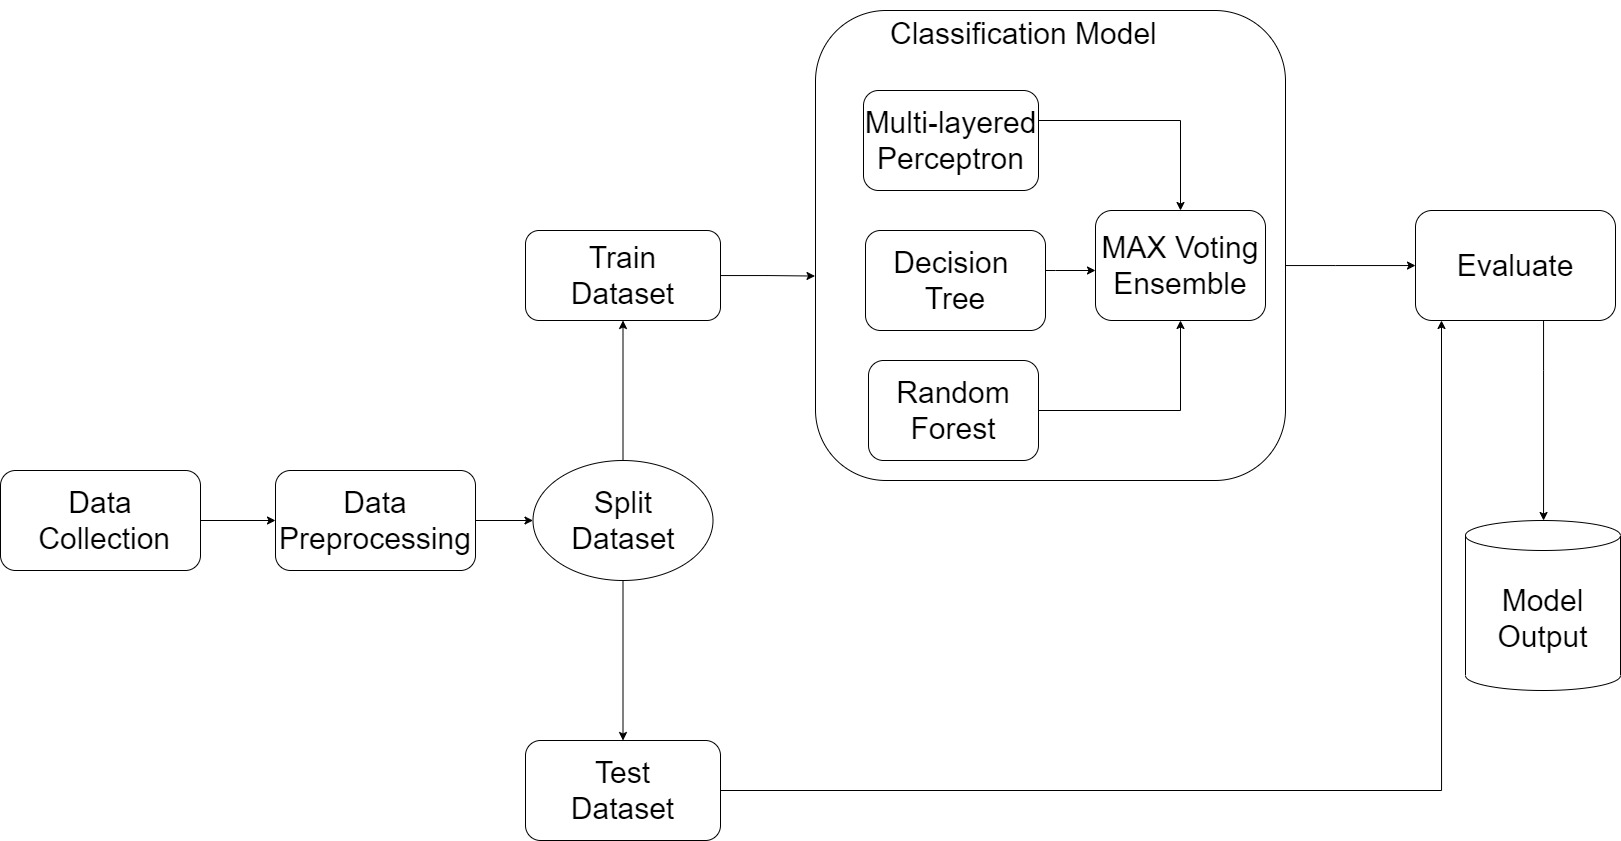
\includegraphics[scale=0.26]{methodo.jpg}
\caption{Block diagram of Thyroid Classification}
\end{figure}
The proposed structure of the project includes different steps. Firstly, thyroid dataset is collected from the Kaggle Website. The dataset has some null values and requires some preprocessing accordingly. After that the dataset is divided into training and testing dataset, training data is used to train the classification models and testing data is used to test and evaluate the perfomance of the system.
\subsection{Data Collection}
Machine learning algorithms are used in the rapid and early diagnosis of thyroid diseases and other diseases, as they are now in a significant position in the health field and help us in diagnosing and classifying diseases and for this reason we have collected our dataset that was found on Kaggle.The data that we have used in our study is a set of data taken from external hospitals and laboratories specialized in analyzing and diagnosing the thyroid diseases. In this dataset, we have found 9172 observations along with 31 attributes. 
\subsection{Data Preprocessing}
The process of pre-processing the data is very important, as good data is crucial for good performance of the models. The pre-processing process is used to reveal the data, as it examines the data with great care. The pre-processing process includes data transformation, cleaning the data, feature selection and data balancing.\\
\begin{figure}[h]
\centering
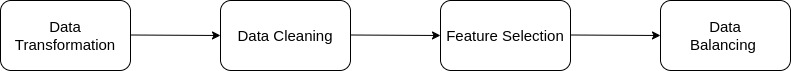
\includegraphics[scale=0.5]{process.jpg}
\caption{Block diagram of Data Preprocessing}
\end{figure}
\par In order to, classify among hypothyroid, hyperthyroid and no condition, sub-diagnosis class labels of hypothyroid and hyperthyroid are transformed as `hypothyroid' and `hyperthyroid' respectively. The dataset had considerable missing values which are addressed to clean the data. Furthermore, dimensional reduction is achieved by using L1 regularization. In this feature selection, linear model is penalised with the L1 norm and SelectFromModel, a meta transformer, alongside the estimater model that assigned importance to each feature is used to select the non-zero coefficients. Machine Learning models can only work with numerical values. For this reason feature encoding is done to transform the categorical values into numerical ones. Finally, to avoid favouring the majority class i.e. no condition by the machine learning models, SMOTE oversampling technique is performed. This balancing technique is ,however, performed to the training dataset only after train-test split on original dataset in order to avoid data leakage.
\subsection{Machine Learning Technique}
The key aim of using machine learning algorithms is to differentiate between three forms of thyroid disease. The first is hyperthyroidism, the second is hypothyroidism, and the third is stable patients who do not have any thyroid issues. In order to facilitate this, different Classification models will be implemented. This is achieved through scikit-learn, an open source machine learning library that also provides various tools for model fitting, data preprocessing, model evaluation, and many other utilities.
\subsubsection{Decision Tree}
A decision tree is one of the most powerful tools of supervised learning algorithms used for both classification and regression tasks. It builds a flowchart-like tree structure where each internal node denotes a test on an attribute, each branch represents an outcome of the test, and each leaf node (terminal node) holds a class label. It is constructed by recursively splitting the training data into subsets based on the values of the attributes until a stopping criterion is met, such as the maximum depth of the tree or the minimum number of samples required to split a node\cite{geeksforgeeks_2017}.

\begin{itemize}
\item Impurity: A measurement of the target variable’s homogeneity in a subset of data. It refers to the degree of randomness or uncertainty in a set of examples. The Gini index and entropy are two commonly used impurity measurements in decision trees for classification tasks.
\end{itemize}

\begin{itemize}
\item Information Gain: Information gain is a measure of the reduction in impurity achieved by splitting a dataset on a particular feature in a decision tree. The splitting criterion is determined by the feature that offers the greatest information gain, It is used to determine the most informative feature to split on at each node of the tree, with the goal of creating pure subsets.
\begin{figure}[h]
\centering
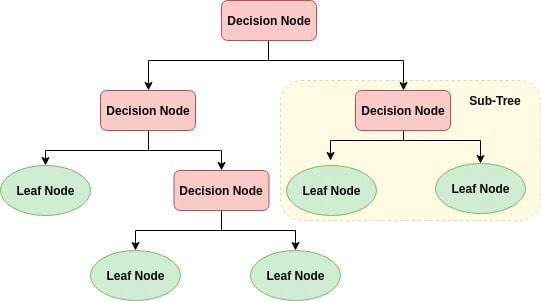
\includegraphics[scale=0.5]{decision_tree.png}
\caption{Decision Tree}
\textit{Source: https://www.numpyninja.com/post/decision-trees-example-in-machine-learning
}
\end{figure} 

\item Entropy:\\
        \textopenbullet\ Entropy is the measure of the degree of randomness or uncertainty in the dataset. In the case of classifications, it measures the randomness based on the distribution of class labels in the dataset.
        \begin{equation}
\textit{\text{Entropy}} = \Sigma - \left( P_i \cdot \log_2{P_i} \right)
\end{equation}
Where, \(P_i\) = Probability of Class\\
\begin{equation}
\textit{\text{Information Gain}} = E(\text{Parent node}) - \sum (W_i \cdot E(\text{Child node}))
\end{equation}
Where, E = Entropy\\
\(W_i\) = Size of Child / Size of Parent 
\item Gini Impurity or index:\\
        \textopenbullet\ Gini Impurity is a score that evaluates how accurate a split is among the classified groups. The Gini Impurity evaluates a score in the range between 0 and 1, where 0 is when all observations belong to one class, and 1 is a random distribution of the elements within classes. In this case, we want to have a Gini index score as low as possible. Gini Index is the evaluation metric we shall use to evaluate our Decision Tree Model.\\ 
\begin{equation}
\textit{\text{Gini index}} = 1 - \sum P_i^2
\end{equation}
\begin{equation}
\textit{\text{Information Gain}} = G(\text{Parent node}) - \sum (W_i \cdot G(\text{Child node}))
\end{equation}
Where, G = Gini index\\
\(W_i\) = Size of Child / Size of Parent  
\end{itemize}
The decision tree model is implemented by importing DecisionTreeClassifier from scikit-learn's tree module. The decision tree model is then trained using the training data. Other utility modules of scikit-learn like metrics is used to evaluate this models performance on test data. Such metrics used to assess the diagnostic performance are Precision-Recall curve, confusion matrix and learning curve. Furthermore, minimal cost complexity pruning is performed by choosing cross validated complexity parameter. 
\subsubsection{Random Forest}
Random forest is a supervised machine learning algorithm that can be used for solving classification and regression problems both. However, mostly it is preferred for classification. It is named as a random forest because it combines multiple decision trees to create a “forest” and feed random features to them from the provided dataset. Instead of depending on an individual decision tree, the random forest takes prediction from all the trees and selects the best outcome through the voting process\cite{awasthi_2020}. 
Now, the question arises why do we prefer random forests over decision trees. So, individual trees are more prone to overfitting but random forests can reduce this problem by averaging the predicted results from each tree.
\begin{figure}[h]
\centering
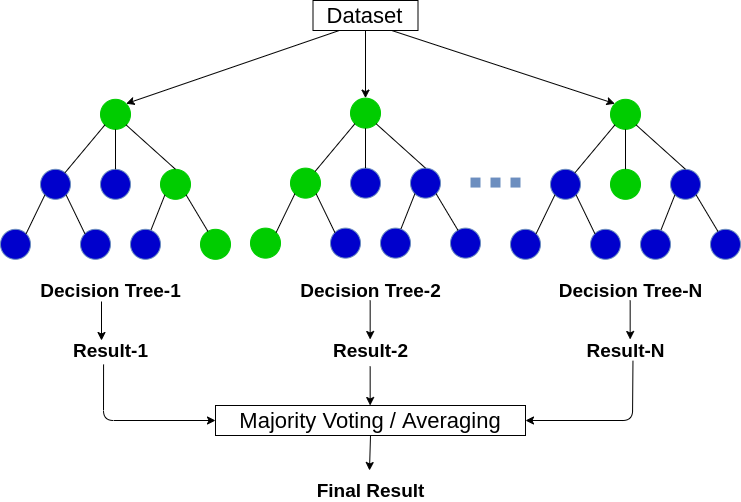
\includegraphics[scale=0.5]{randomforest.png}
\caption{Working diagram of Random Forest}
\textit{Source:https://datamahadev.com/random-forests-in-machine-learning-a-detailed-explanation/}
\end{figure}

Random Forest  is implemented by importing RandomForestClassifier from ensembled module of scikit-learn. The model is initialized with 50 base estimators and trained on the training dataset. Like decision tree, minimal cost complexity for random forest is performed. Likewise, the model is evaluated to diagnose its performance.
\subsubsection{Support Vector Machine(SVM)}
Support Vector Machine(SVM) constructs a Hyperplane or set of hyperplanes in a high- or infinite-dimensional space, which can be used for classification, regression, or other tasks.The Support Vector Machine (SVM) stands as a supervised machine learning algorithm with applications in both
classification and regression tasks. While SVM is versatile enough to handle regression problems, its optimal
utility lies in the domain of classification. The central objective of the SVM algorithm involves the identification
of a hyperplane within an N-dimensional space that distinctly segregates the data points. The dimensionality of
this hyperplane is contingent upon the quantity of input features. In scenarios where the input features number
two, the hyperplane is represented as a line. For instances with three input features, the hyperplane assumes the
form of a 2-dimensional plane. However, the visualization of hyperplanes becomes progressively intricate as the
number of features surpasses three\cite{pralhad}.

\begin{figure}[h]
\centering
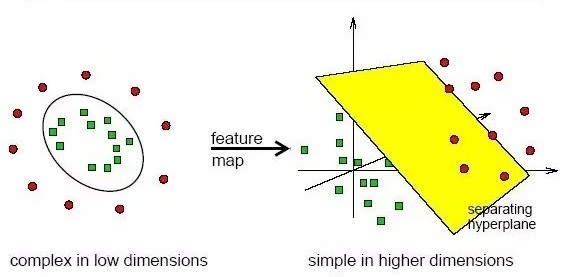
\includegraphics[scale=0.65]{svm.png}
\caption{SVM}
\textit{Source:https://www.dtreg.com/solution/support-vector-machines}
\end{figure}

\subsubsection{Multi-Layer Perceptron(MLP)}
Multi-Layer Perceptrons, a fundamental type of neural network, are vital tools in supervised learning, predominantly used for complex pattern recognition, classification, and regression tasks. An MLP consists of multiple layers: an input layer, one or more hidden layers, and an output layer. Each layer is made up of nodes, or neurons, which are interconnected and apply activation functions to their inputs.
Initially, the weights of the connections between neurons are randomly assigned. Each connection between neurons has an associated weight, which determines the strength of the connection. Additionally, each neuron has a bias, which helps in adjusting the output.he information flows through the network in a forward direction during the training process. 
The input data is fed into the input layer, and the output is obtained from the output layer. The computations are performed layer by layer, using the weights and biases.\par
\begin{figure}[h]
\centering
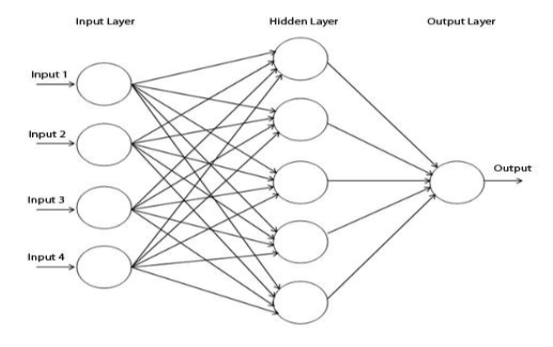
\includegraphics[scale=0.65]{tree.png}
\caption{MLP structure}
\textit{Source:
https://www.researchgate.net/publication/329277388 \\ \_Application\_of\_Multilayer\_Perceptron\_MLP\_for\_Data\_Mining\_in\_Healthcare\_Operations}
\end{figure}
If a multilayer perceptron has a linear activation function in all neurons, that is, a linear
function that maps the weighted inputs to the output of each neuron, then linear algebra
shows that any number of layers can be reduced to a two-layer input-output model. In MLPs
some neurons use a nonlinear activation function.The ReLU activation function is widely used in neural networks due to its simplicity and effectiveness. It is defined as:\\
$f(x)$ $=$ $max(0,x)$\\
The ReLU function returns the input x if it is positive, and zero otherwise. It introduces non-linearity to the model, allowing it to learn and represent complex patterns.
Each connection between neurons has an associated weight, which determines the strength of the connection.\\
The difference between the predicted output and the actual target is quantified using a loss function; log-loss in case of classification. The goal during training is to minimize this loss.
During training, the network learns by adjusting its weights and biases to minimize the difference between its predicted output and the actual target values. This process is known as backpropagation. Gradient descent is often used as the optimization algorithm to update the weights and biases in the direction that minimizes the error.\\
$New Weight = Old Weight - Learning Rate * Gradient$\\
Training is typically done over multiple passes through the entire dataset, known as epochs\cite{inproceedings}.

MLP is implemented by importing MLPClassifier from neural\_network module in scikit-learn. The model is initialized by allowing 500 maximum iterations followed by strength of the L2 regularization term of 0.076, and trained on the training dataset. The model is evaluated in the similar fashion as previous model, meanwhile the learning curve for MLP depicts the loss function at each epoch. This shows how the optimization in MLP is iterating until convergence.

\subsection{Split Dataset}
An important phase in the model development process is splitting the facts for system mastery models. It entails breaking up the available dataset into training and testing datasets.
%\subsubsection{Train Dataset Split}
The testing out set is used to evaluate the model's overall performance while the training set is used to teach the model. The typical cut up is 20–30\% for testing out and 70–80\% for training, but this might change based on the size of the dataset and the specific use case. 
%\subsubsection{Test Set Split}
The testing set provides an objective assessment of the generalizability of our model. We assess our model's performance on the testing set once it has been fully trained and tuned using the training and validation sets. This phase accurately predicts how well our model will perform on new thyroid patient samples that it hasn't seen before.
\subsection{Train Model}
Training a machine learning model involves the process of feeding data to the model, adjusting its internal parameters, and optimizing its performance. In the context of thyroid patient classification, the model will learn from the input features and their corresponding labels during this process. The specific training algorithm and duration depend on the chosen model and complexity of the data.
\subsection{Model validation}
Model validation is the task of evaluating whether a chosen model is appropriate or not. The significance of a correct medical diagnosis necessitates specific considerations when validating a machine learning model for thyroid illness categorization.
\subsection{Model Output}
We use streamlit which allows us to display descriptive text, model outputs, and enter new inputs through the User-Interface for classification of thyroid. Inorder to save the model trained, module called pickle is used, which can be defined as a module in Python used for serializing and de-serializing Python objects. This converts Python objects like lists, dictionaries, etc. into byte streams (zeros \& ones).
\section{Development Model}
The Incremental model, which is a mixture of waterfall and iterative development approach is opted, as the project demands few requirements and is fairly simple. As the name suggests, the major objective is focused as the first increment of the project. The activities in this model are completed iteratively and each outcome acts as an input for the next phase, thus increments are developed in such a way.
\subsection{Requirement Specification}
The final product can be divided into two parts: the frontend and the backend. The frontend shall be a simple page where users can input a few specific hormones (assuming the user has measured these hormones prior to using the product), and obtain their thyroid condition. Whereas, the backend consists of training our models evaluating them before exporting as a pickle file.
\subsection{Development and Implementation}
The project has the architecture close to any other ML projects, i.e. EDA --$>$ pre-processing --$>$ model training --$>$ save model. The product is written using python programming language and jupyter notebook. The interface for the use of the product is rather simple as the only requirement is classification of thyroid, which is achieved through the use of the streamlit framework.
\begin{figure}[h]
\centering
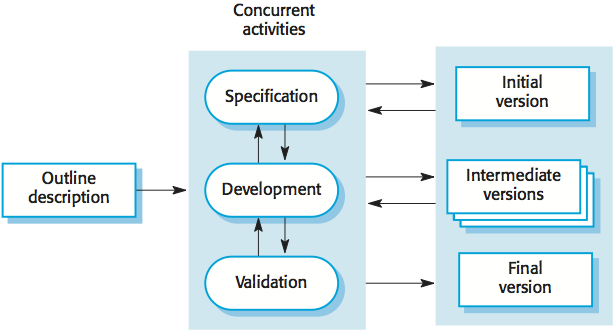
\includegraphics[scale=1]{incremental.png}
\caption{Incremental Development Model}
\textit{Source: https://copyprogramming.com/howto/the-best-sdlc-model-to-deploy-in-software-dev}
\end{figure}
\subsection{Verification and Validation}
In order to approve that the product meets its defined objectives, verification and validation is exercised. This involves Meetings and Code reviews. However, considering the imbalance of data in our thyroid dataset there are chances our model overfitting. Thus, we implemented balancing methods to handle the imbalanced data. 
The code itself is verified with inspections and walkthroughs among the group and even by external parties. Finally, the product is verified by testing its classification prediction on the testing split of dataset.
\subsection{Increments}
As discussed earlier the project went through several increments. The first increment solely focuses on the major requirement, developing models for the required classification. The further increments are focused on evaluation of the models, exporting the best model, developing a front-end for the product.

\section{Evaluation Criteria}
Upon the successful construction of a system model, it undergoes training using the training dataset sourced from
the standardized dataset.The effectiveness of the system's performance is assessed by Accuracy, Precision, Recall, and F1 score
.\\
\textbf{Accuracy:}\\
The ratio of true positives and true negatives to all positive and negative observations is the definition of model accuracy, a performance statistic for machine learning models.\\
$Accuracy =$ $\frac{TP + TN}{TP + FN + TN + FP}$\\
\textbf{Precision:}\\
The percentage of labels that were correctly predicted positively is represented by the model precision score.\\
$Precision =$ $\frac{TP}{TP + FP}$\\
\textbf{Recall:}\\
The model's ability to properly forecast the positive out of actual positives is measured by the model recall score.\\
$Recall =$ $\frac{TP}{TP + FN}$\\
\textbf{F1 Score:}\\
The F1 score combines precision and recall using their harmonic mean, and maximizing the F1 score implies
simultaneously maximizing both precision and recall.\\
$F1 Score =$ $\frac{2*Precision*Recall}{Precision+Recall}$\\

\section{System Diagrams}
Thyroid Detection System prompts the user to enter different data from their medical test report such as age, sex, T3, T4, TSH values for the system to classify whether they are suffering from hypothyroidism/hyperthyroidism or not. Use of different maching learning models such as Decision Tree, Random Forest, MLP aids in thyroid classfication so the user has better understanding of their thyroid health. If the user doesnot have all the required data from the medical test report, the system prompts the user to enter their details for their thyroid classification.
%\newpage
\subsection{Usecase Diagram}

\begin{figure}[h]
\centering
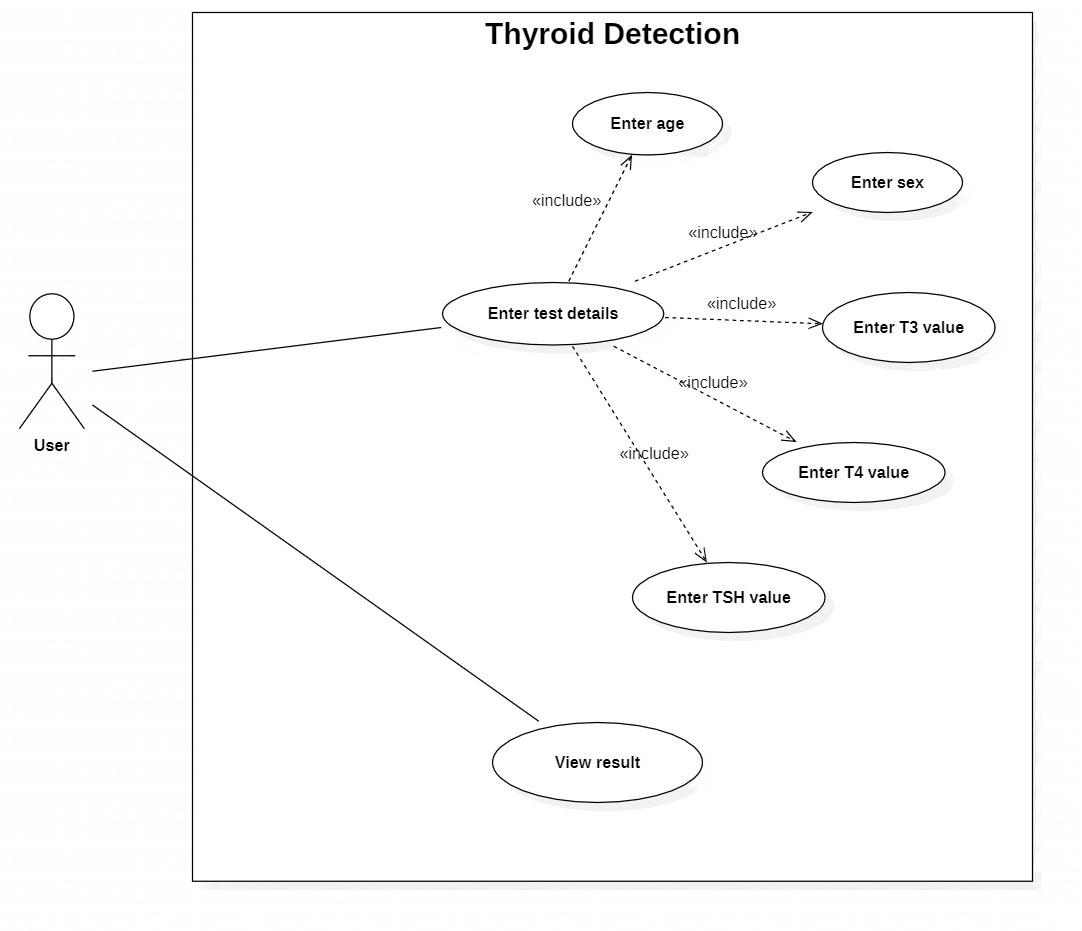
\includegraphics[scale=0.5,width=14cm]{usecase.png}
\caption{Usecase Diagram}
\end{figure}
%\newpage
\subsection{DFD}
\begin{figure}[h]
\centering
\includegraphics[scale=0.75]{dfd1.jpg}
\caption{DFD diagram}
\end{figure}
\subsection{Class Diagram}
\begin{figure}[h]
\centering
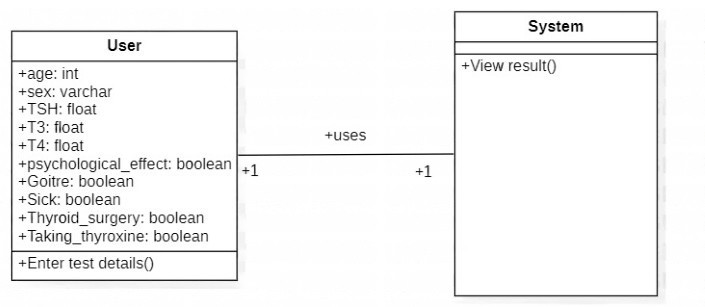
\includegraphics[scale=0.5]{class.png}
\caption{Class diagram}
\end{figure}
%\newpage
\subsection{Activity Diagram}
\begin{figure}[h]
\centering
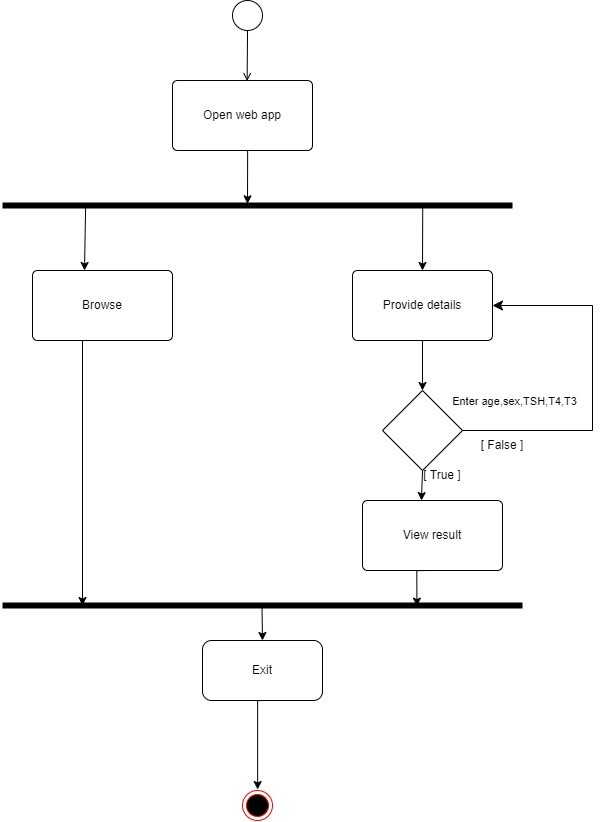
\includegraphics[scale=0.5]{activity.jpg}
\caption{Activity Diagram}
\end{figure}

\chapter{Result And Discussion}
%\addcontentsline{toc}{chapter}{Result And Discussion}
\section{Preprocessing}
As described in the proposed methodology, the feature selection and feature preprocessing yield the balanced thyroid disease classification dataset. The majority of the classification count is categorized as ``no condition". The ``no condition" means that the data sample is not categorized as any other classes like hyperthyroid, hypothyoid, binding proteins, general health, replacement therapy, antithyroid treatment, or miscellaneous meaning the subject is healthy with no thyroid conditions.
For the condition hyperthyroid, the diagnosis classes were hyperthyroid(A), T3 toxic(B), toxic goitre(C), secondary toxic(D) and their count was 147, 21, 6 and 8 respectively. The low counts of this diagnosis class were remapped into hyperthyroid class which would make easier for thyroid classification. Similarly, the same was performed for hypothyroid condition where the subclasses were remapped into hypothyroid.\\
The diagnosis classes for binding protein were increased and decreased binding protein whose count were 346 and 30 respectively. The count for the general health condition was 436. The diagnosis classes for replacement therapy were underreplaced, consistent with replacement therapy, and overreplaced whose counts were 111, 115 and 110 respectively. The diagnosis classes for antithyroid treatment condition were antithyroid drugs, I131 treatment and surgery with counts 14, 5 and 14 respectively. The miscellaneous condition and its classes with count were; discordant assay result - 196, elevated TBG - 85, elevated thyroid hormones - 0. For no thyroid condition the count was 6771.\\
The dataset consists of 9173 patient records out of which 6771 are normal patient records, and notable conditions include primary hyperthyroid 233 and compensated hypothyroid with 359 patients. Since the number of samples for other classes were not significant, we remapped the dataset and selected only hyperthyroid, hypothyroid and no thyroid conditions while other classes with low instances were not considered. Thus, we have a dataset of 7542 instances with 593 hypothyroid cases and 182 hyperthyroid cases.

\begin{figure}[h]
\centering
%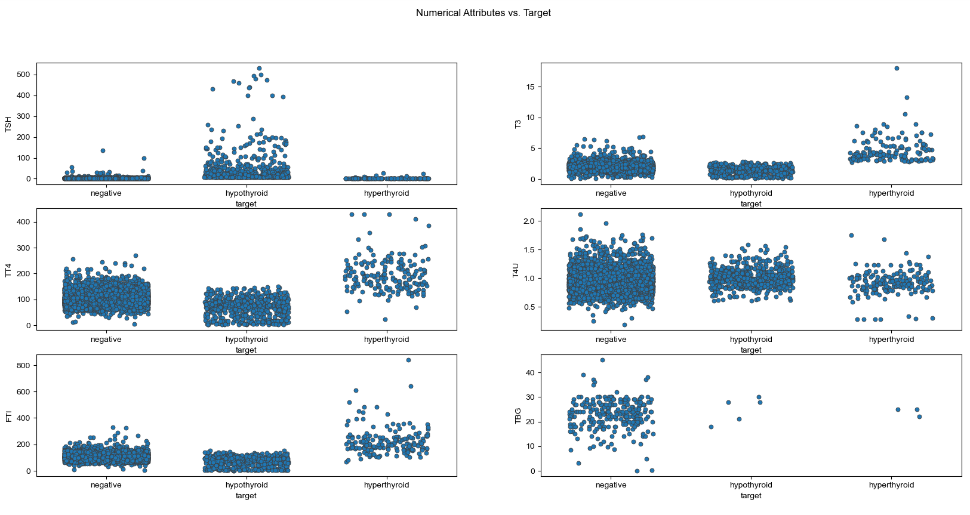
\includegraphics[scale=0.5]{strip.png}
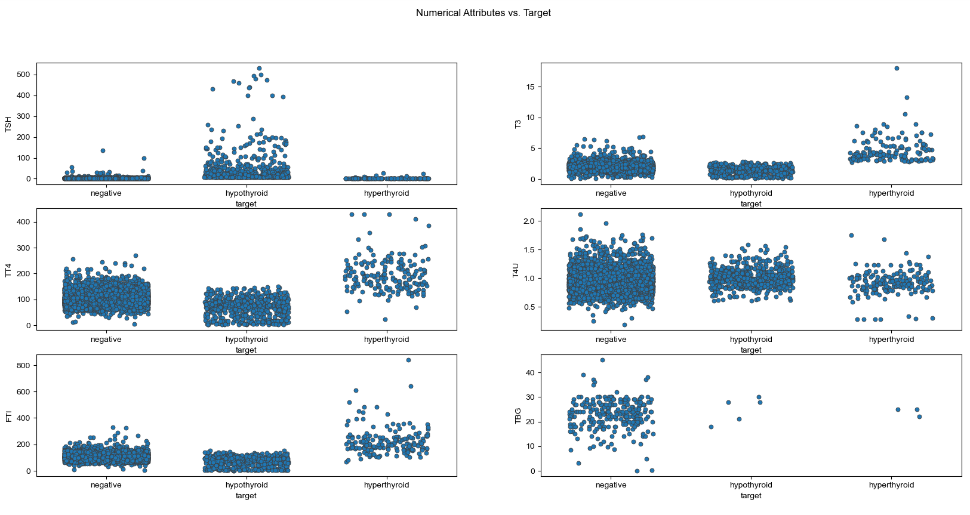
\includegraphics[height=10cm, width=15cm]{strip.png}
\caption{Strip plot: Numerical Attributes vs Target}
\end{figure}
\newpage
On observing the above strip plot, the attributes TSH, TT4, T3, FTI can be good candidate to effectively classify thyroidism.Furthermore, the attributes TBG has less instances which we addressed in data cleaning.

\subsubsection{Data Cleaning}
The dataset has tons of missing values so we analyzed all the missing values from the dataset. 7287 instances of TBG, about 96.5\% of total were found to be missing, so we dropped the TBG attribute as a whole. Also for T3, out of 2209 instances, 29.2\% of data was found to be missing but we had observed that T3 is an important attribute for classification so we didnot completely drop it and performed median imputation. Same imputation was done for other missing features. After this our dataset is clean with no missing/null-values.
%\section{Result}

\begin{figure}[h]
\centering
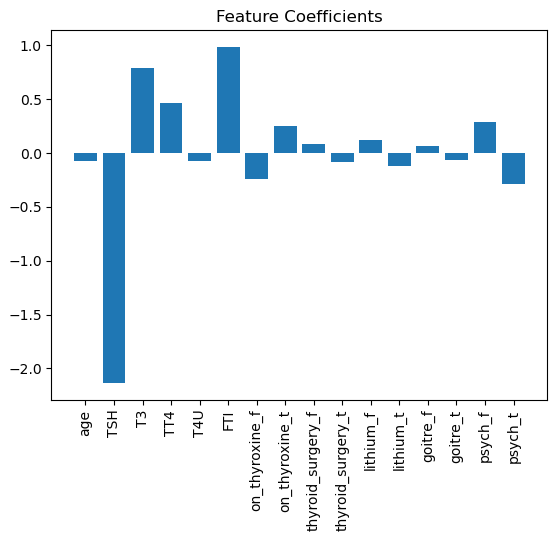
\includegraphics[scale=0.75]{featureselect.png}
\caption{Feature Selection}
\end{figure}

\subsubsection{Feature Selection}
L1 regularization was used for feature selection. L1 regularization is commonly used in machine learning to enhance model generalization and perform
feature selection by penalizing the absolute values of the coefficients in logistic regression. The loss function with L1 regularization is modified by adding the L1 norm of the coefficients(weights) to the standard loss term:
\begin{equation}
\begin{aligned}
J(\theta) &= \text{Loss}(\theta) + \lambda \sum_{i=1}^{n} |\theta_i| \\
\end{aligned}
\end{equation}Here, $J$($\theta$) is the regularized loss funtion. $Loss$($\theta$) is the original loss(e.g., categorical cross-entropy loss for multi-class classification),$\lambda$ is the regularization parameter, \textit{n} is the number of features, and \( \theta_i \) represents the coefficients.\\
The L1 regularization term, $\lambda$ $\sum_{i=1}^{n} | \theta_{i} | $ introduces a penalty for having non-zero coefficients. As a result, during the optimization process, some of the coefficients are driven to exactly zero, effectively leading to feature selection\cite{ng}.
After feature selection the relevant features that were selected are: age, sex, TSH, T3, TT4, T4U, FTI, On\_Thyroxine, Thyroid\_Surgery, sick, goitre, psych and Target.\\
\begin{table}[h]
\caption{Thyroid disease attributes \& dataset info}
\begin{tabular}{p{2.5cm}  p{4cm}  p{3.2cm}  p{1.5cm} p{1.5cm}}
\hline
Attribute & Description & Domain of Value & Non-Null & DType \\
\hline
Age & Age in years & 1 to 97 & 7542&Float64\\\\
Sex & Sex & Female(F) Male(M) & 7542 & object\\\\
TSH & Thyroid-stimulating hormone & 0.01 to 530 \(\mu\)IU/ml & 7542&Float64\\\\
T3 & Triiodothyronine & 0.05 to 18.00 ng/mL& 7542&Float64\\\\
TT4 & Total thyroxine & 2.00 to 600.00 ng/mL& 7542&Float64\\\\
T4U & Thyroxine Uptake & 0.17 to 2.33 & 7542 & Float64\\\\
FTI & Free Thyroxine Index & 1.40 to 881.00 & 7542 & Float64\\\\
On\_Thyroxine&  Taking thyroxine tablet & True(t) False(f) & 7542&object\\\\
Thyroid\_Surgery& Undergone thyroid related surgery&True(t) False(f) & 7542&object\\\\
sick & Currently ill&True(t) False(f)&7542&object\\\\
goitre & Enlarged thyroid gland& True(t) False(f)  & 7542&object\\\\
psych & Thyroid related psychological symptoms&True(t) False(f)&7542&object\\\\
Target & Thyroid Disease & Hyperthyroid Hypothyroid Negative & 7542 & object\\\\
\hline
\end{tabular}
\end{table}\\
The categorical features are encoded as most machine learning models only accept numerical variables, thus preprocessing the categorical variables was a necessary step.
\newpage
\newpage
\section{Model Training}
Firstly, we trained Decision Tree with default parameters. Even though its predictions were optimistic for the testing dataset, it was clearly overfitting. The model was complex due to it trying to fit all the training dataset and couldn't generalize well for new datas.This was evident as the loss on test was high compared to train dataset.\\
The formula for categorical log loss is:
\begin{equation}
\begin{aligned}
\text{CategoricalLogLoss} &= -\frac{1}{N} \sum_{i=1}^{N} \sum_{j=1}^{M} y_{ij} \log(p_{ij}) \\
\end{aligned}
\end{equation}
Where: \\
\textit{N} is the number of samples or instances in the dataset. \\
\textit{M} is the number of classes. \\
$y_{ij}$ is a binary indicator (0 or 1) if class label \textit{j} is the correct classification for instance \textit{i}. \\
$p_{ij}$ is the predicted probability that instance \textit{i} belongs to class \textit{j} \cite{cross_entropy}. 
\begin{figure}[h]
\centering
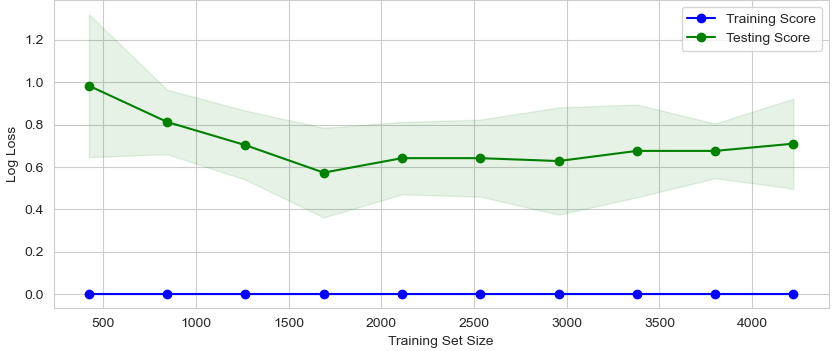
\includegraphics[scale=0.5]{learning.png}
\caption{Overfitting Decision Tree}
\end{figure}\\
When it comes to medical datasets, it is normal that the datas on normal patients dramatically outweighs actual cases of illness. Same was the case for our thyroid dataset so oversampling technique namely SMOTE, was performed.
Now, another decision tree model was trained on balanced dataset. This model was not complex thus could generalize to new unseen datas.
\begin{figure}
\centering
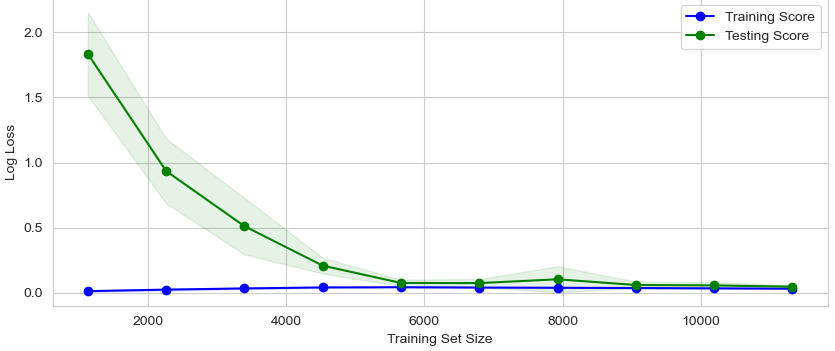
\includegraphics[scale=0.5]{learn.png}
\caption{Decision Tree on Balanced Dataset}
\end{figure} \par
Other models for classifications were tested i.e. SVM, RF, and MLP. However, the performance of SVM was subpar compared to other models evaluated. Remanining models, RF and MLP, worked well on the balanced dataset. Since, we need to classify thyroid conditions, we had to make sure the models are correctly classifying positive instances, Hypothyroid and hyperthyroid. Thus, Recall is the primary focus of criteria for our models(Low False-Negatives). Generally, recall improves at the expense of precision or precision improves at the expense of recall\cite{gordon1989recall}. While, balancing the dataset, recall was improved while trading-off precision, we had to make sure the trade-off in precision is not that large(High False-Positives).
\\
\begin{table}[h]
\caption{Performance of the Models}
\begin{tabular}{p{3.5cm} p{2cm} p{2cm} p{2cm} p{2cm}}
\hline
 & Accuracy(\%) & Precision(\%) & Recall(\%) & F1-Score(\%) \\
\hline
Decision tree on imbalanced dataset & 98.674 & 90.152 & 90.512 & 90.331 \\\\
Decision tree on balanced dataset & 98.188 & 85.168 & 96.620 & 89.793 \\\\
SVM & 92.930 & 69.039 & 91.292 & 74.946 \\\\
RF & 97.791 & 83.467 & 97.830 & 89.174 \\\\
MLP & 96.774 & 80.868 & 96.494 & 87.372 \\\\
Ensembled Model & 98.011 & 84.966 & 97.233 & 90.106 \\\\
\hline
\end{tabular}
\end{table}
 This low precision of SVM, compared to other models, was the sole reason to not consider it for the final Ensembled model. Since three models are performing well, we employed Soft Max Voting ensemble model which can incorporate the predictions made by all three models to generate best possible result. This ensembled model has high recall score, while balancing out the precision-recall trade-off; it has the highest F1-score of 90.106\%.\\
\begin{figure}[h]
\centering
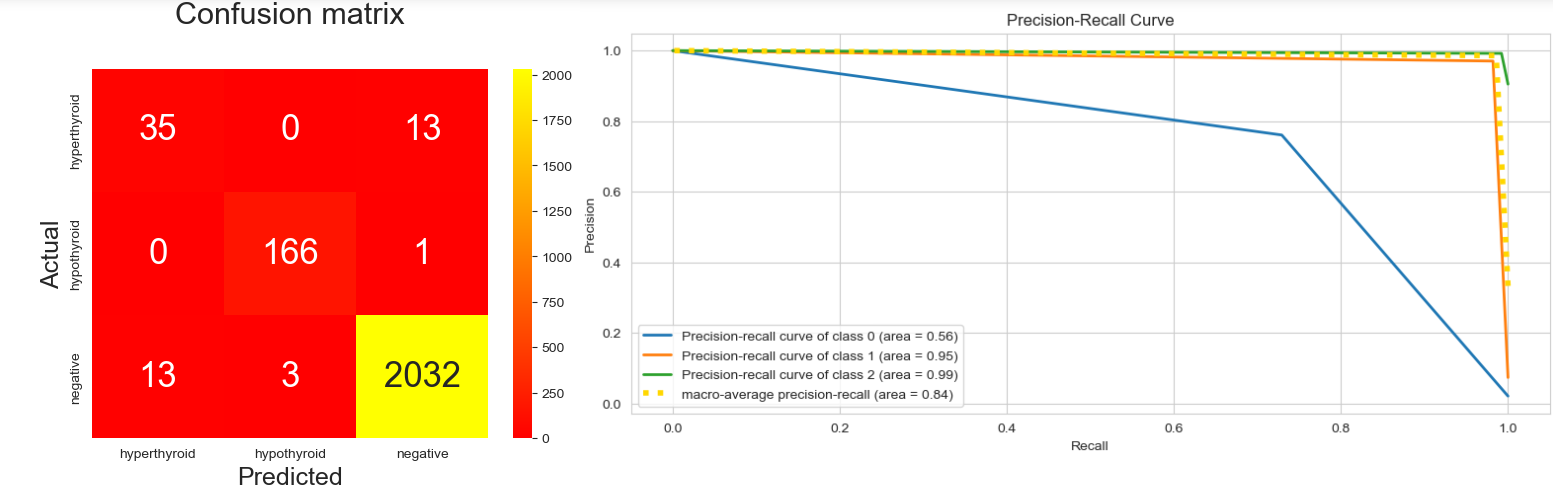
\includegraphics[scale=0.35]{unbalanced.png}
\caption{Evaluation of Unbalanced Decision Tree}
\end{figure}

\begin{figure}[h]
\centering
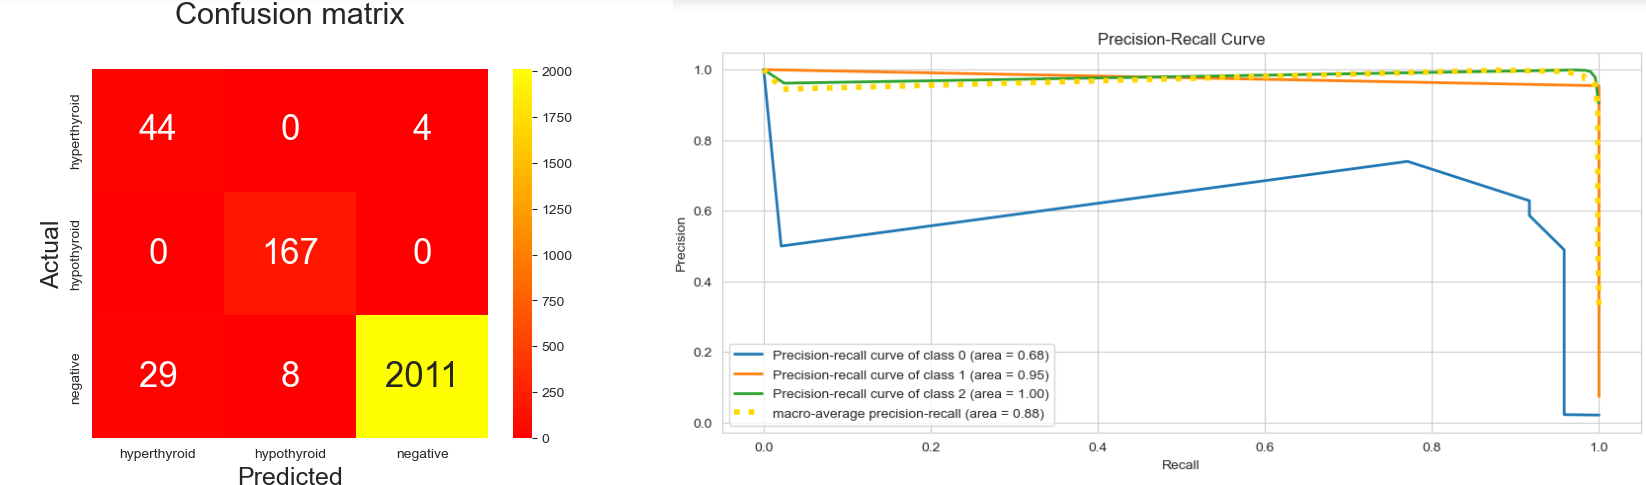
\includegraphics[scale=0.5, width=14cm]{balanced.png}
\caption{Evaluation of Balanced Decision Tree}
\end{figure}

\begin{figure}[h]
\centering
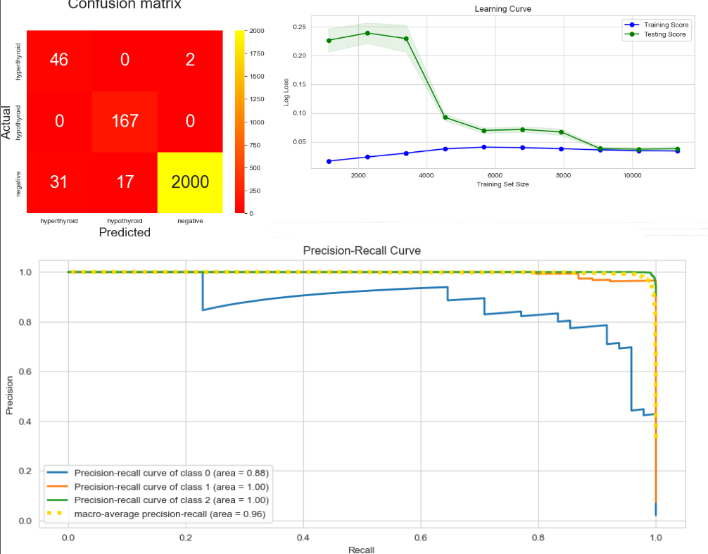
\includegraphics[scale=0.5,  height=10cm, width=14cm]{random.png}
\caption{Evaluation of Random Forest}
\end{figure}

\begin{figure}[h]
\centering
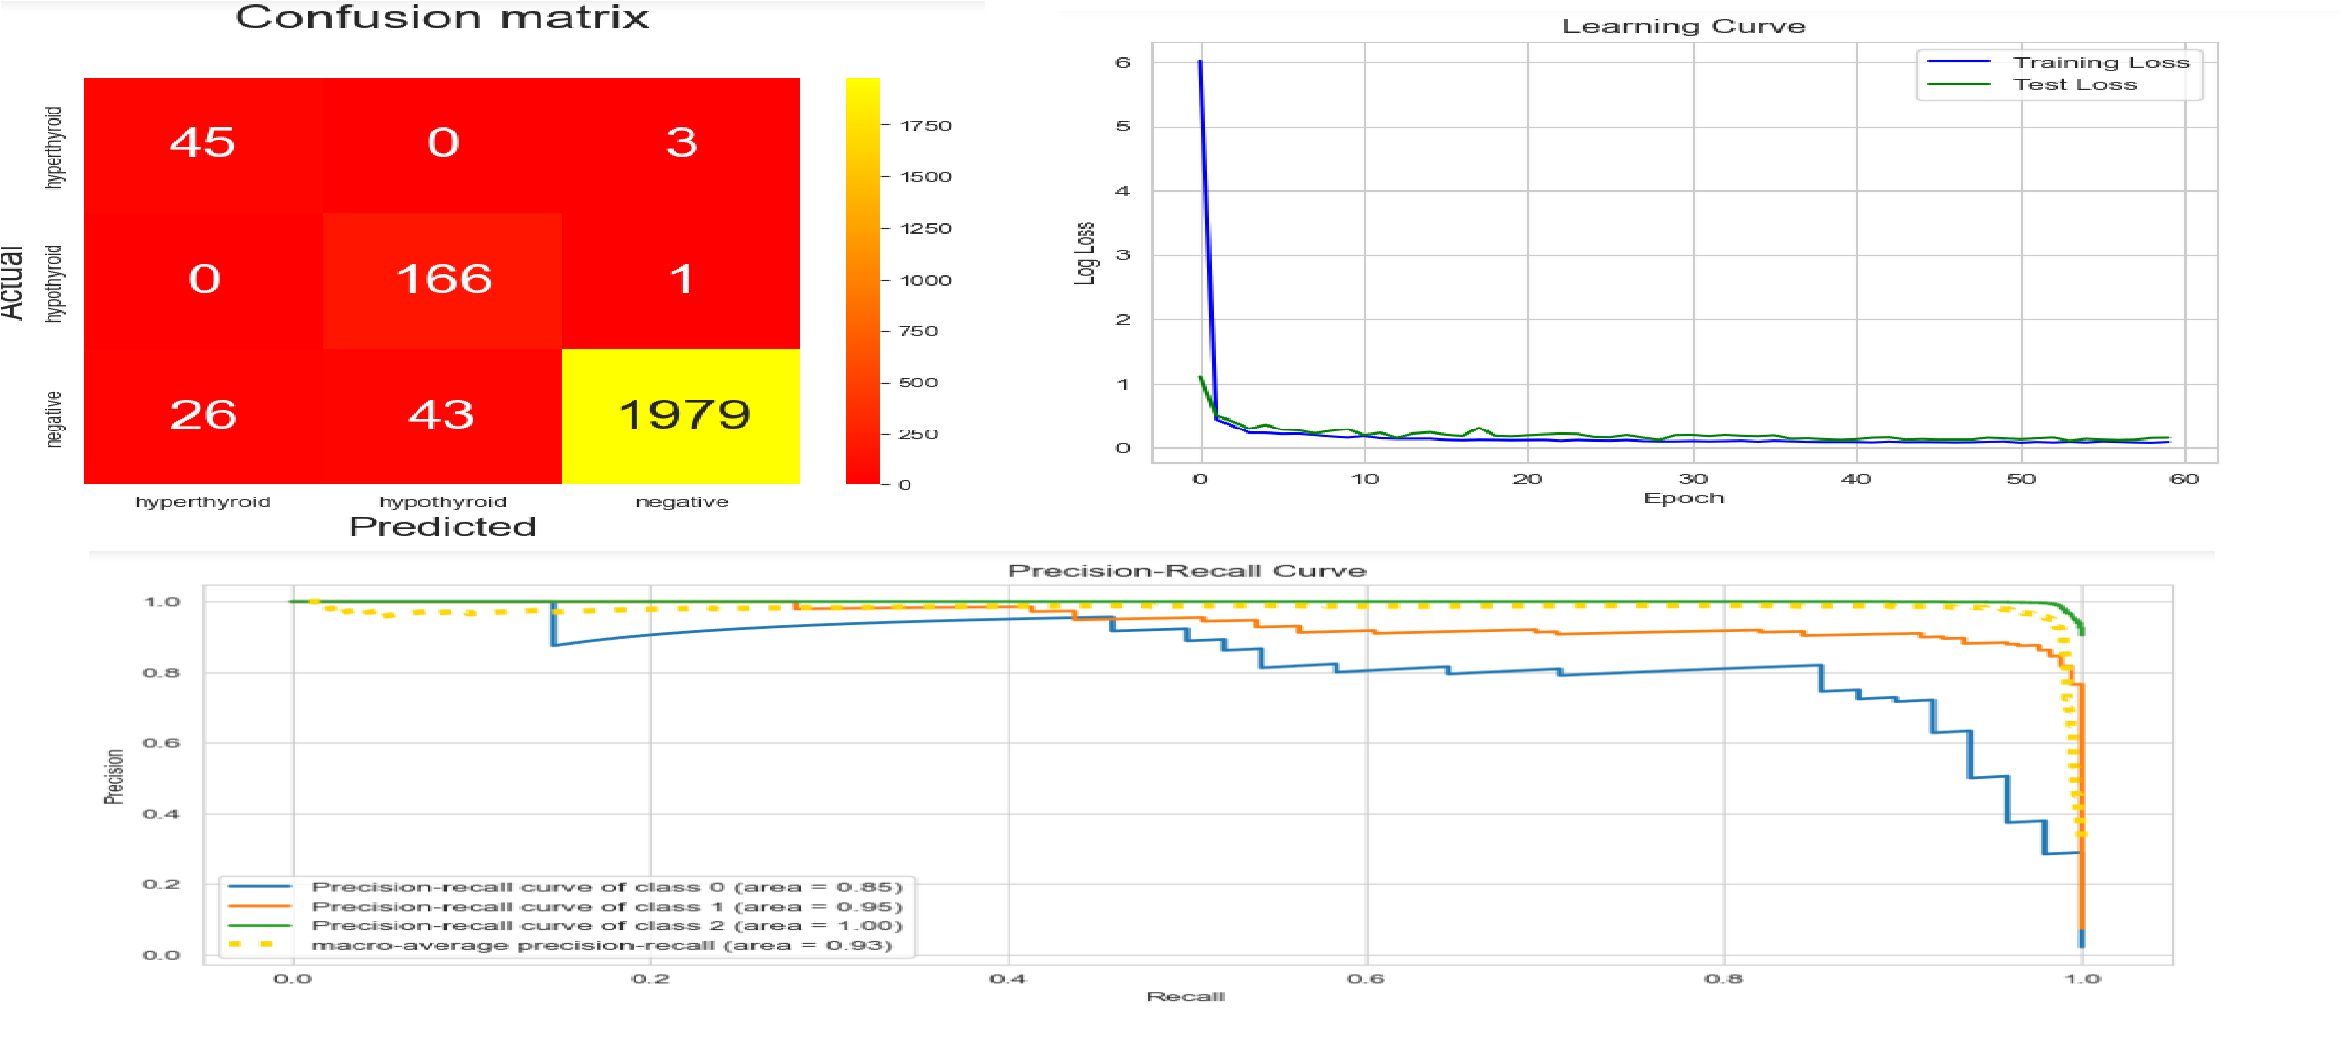
\includegraphics[scale=0.5, height=10cm, width=15.5cm]{multil.png}
\caption{Evaluation of MLP}
\end{figure}

\begin{figure}[t]
\centering
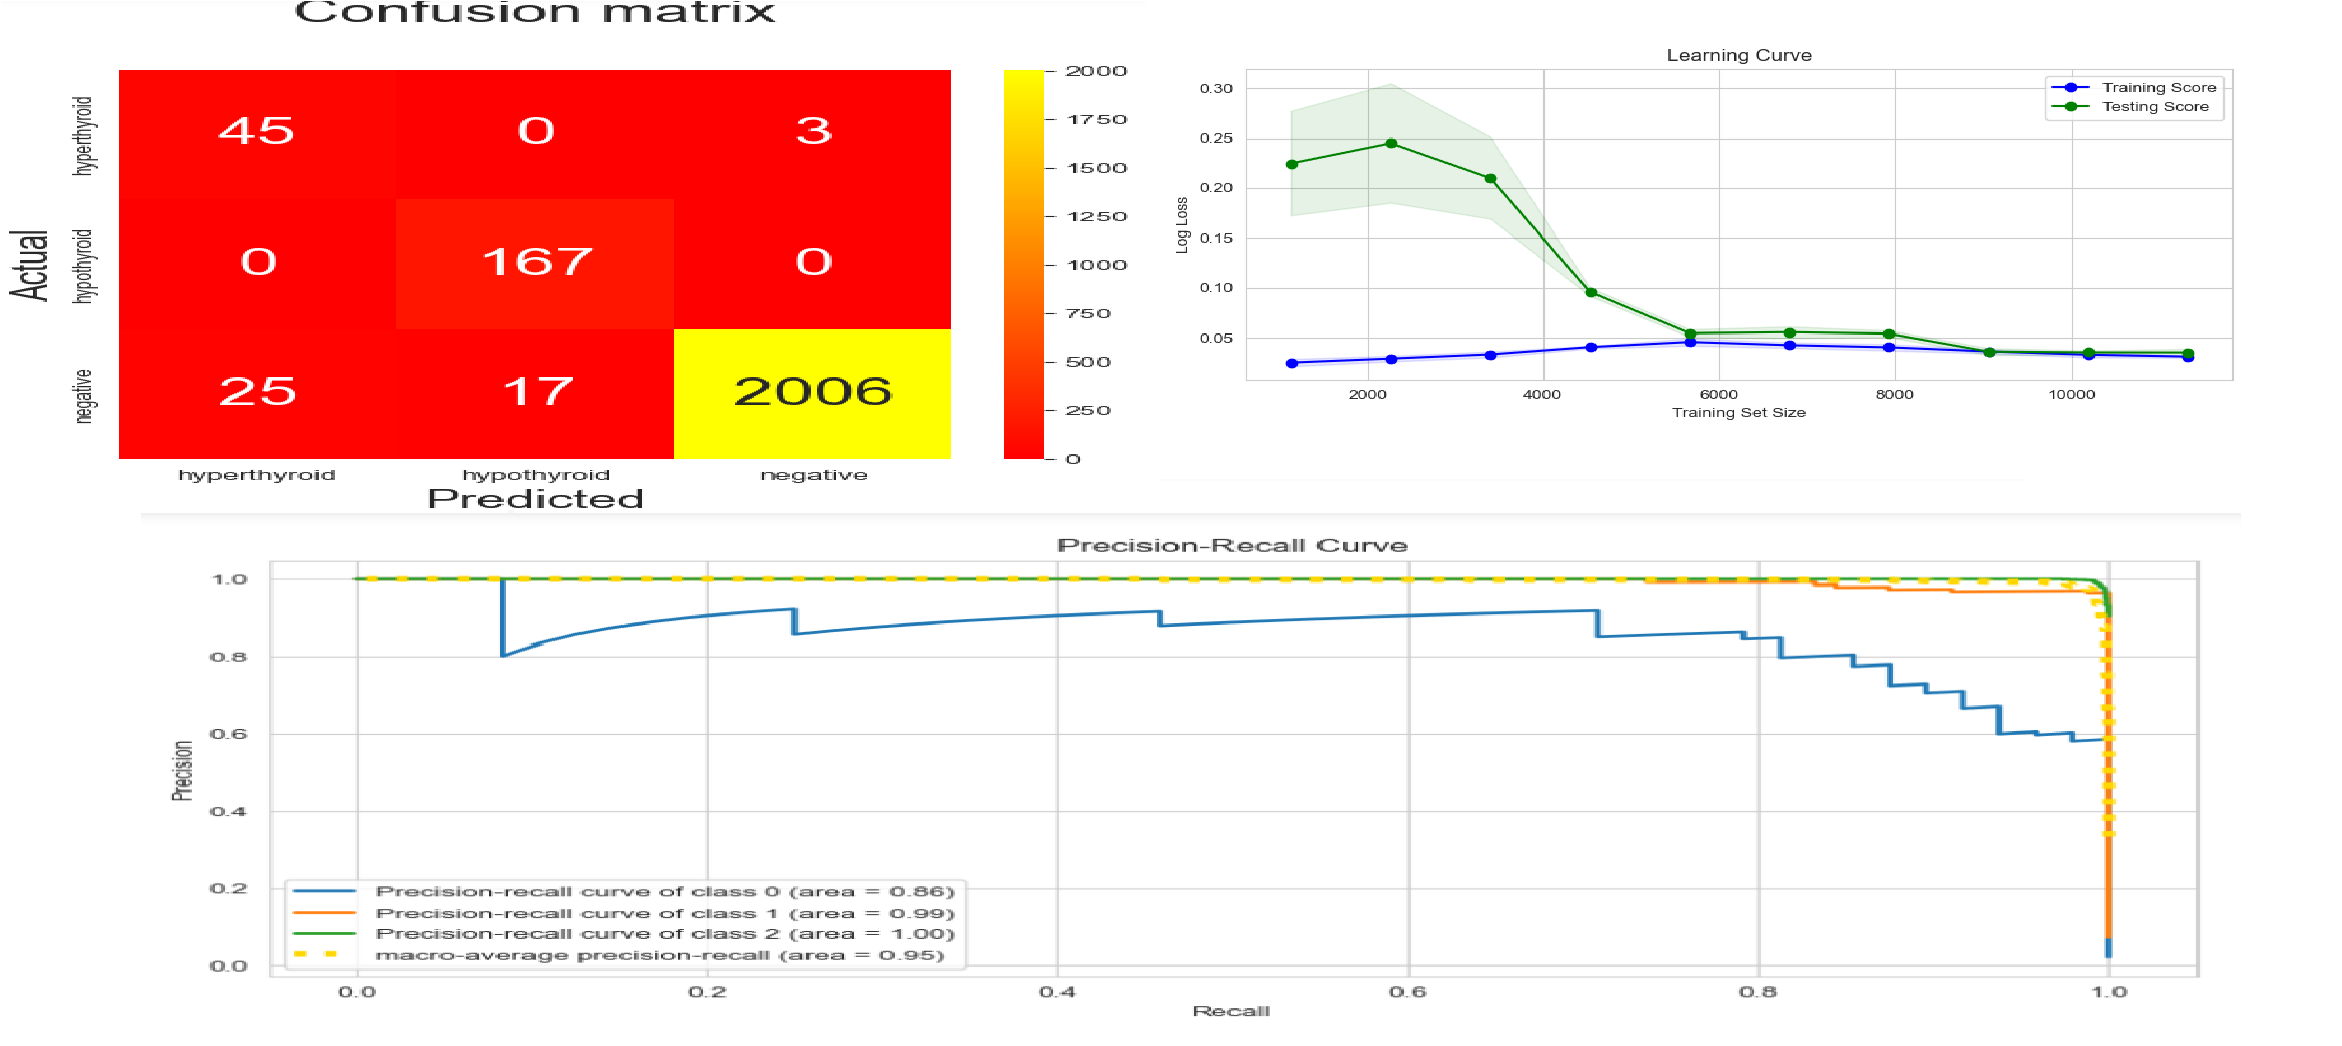
\includegraphics[scale=0.45, height=10cm, width=15cm]{ensemble.png}
\caption{Evaluation of Ensemble}
\end{figure}

After finalizing the ensemble model as our model to classify thyroids for early diagnosis, we exported this model as a pickle file. This model as a pickle file is made to predict the classifications of new datas entered by the final system's user. We prepared a simple and interactive web-app through the use of streamlit for users to interact with the system.\\
\chapter{Conclusion And Future Enhancements}
%\addcontentsline{toc}{chapter}{Conclusion and Future Enhancements}
\section{Conclusion}
Since thyroid conditions are problem plaguing the world, thyroid conditions classification is a matter of great importance. 
The project focused on the classification of thyroid disorders, with specific emphasis on hyperthyroidism, hypothyroidism and no thyroid conditions. Through the use of machine learning models, the project aimed to accurately differentiate between these conditions based on relevant features extracted from thyroid function tests. The algorithms' recall is one of the key factors when evaluating our models, as it is concerned with the positive classes' classification, hypothyroidism and hyperthyroidism. Ultimately, our model ensembled from classification models showed promising result with high recall and balanced trade-off with precision. The development of such a classification system holds great potential for aiding clinicians in diagnosing thyroid disorders more efficiently and effectively, ultimately leading to better patient outcomes.
\section{Future Enhancements}
\begin{itemize}
\item Implement a mechanism for the system to continuously learn from new data and update its classification models over time, ensuring that it remains accurate and up-to-date with the latest medical knowledge.
\item Implement features for long-term monitoring of patients with thyroid disorders, such as tracking changes in thyroid function over time and adjusting treatment plans accordingly.
\item Develop tools or features to engage patients in managing their thyroid health, such as educational resources or reminders for follow-up appointments and medication adherence.
\end{itemize}
\newpage
%\section{Schedule}

%\begin{figure}[ht]
 %   \centering
  %  \includegraphics[scale=0.5]{photo/ganttchart.png}
   % \caption{Gantt Chart}
    %\label{fig:my_label}
%\end{figure}



%Reference
\renewcommand{\bibname}{REFERENCES} % Change heading to References
\bibliographystyle{IEEEtran} % to use IEEE Format for referencing
\bibliography{library} % specify the .bib file containing reference information 
\addcontentsline{toc}{chapter}{References} % to add references in TOC

%Comment this Chapter if you do not need to include Appendix.

%\addcontentsline{toc}{chapter}{Appendix}
 \chapter*{ANNEX}
 \addcontentsline{toc}{chapter}{Annex}
 
\begin{figure}[ht]
\centering
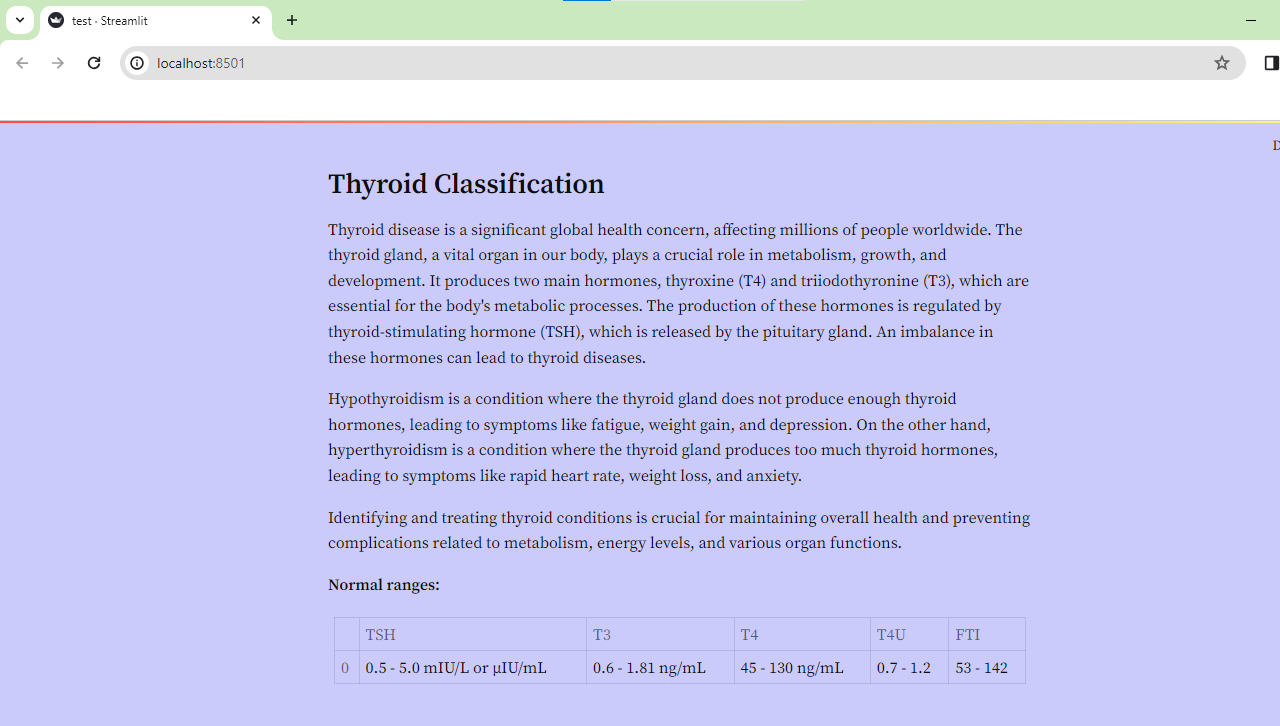
\includegraphics[scale=0.4]{result1.png}
\caption{Result 1}
\end{figure}

\begin{figure}[h]
\centering
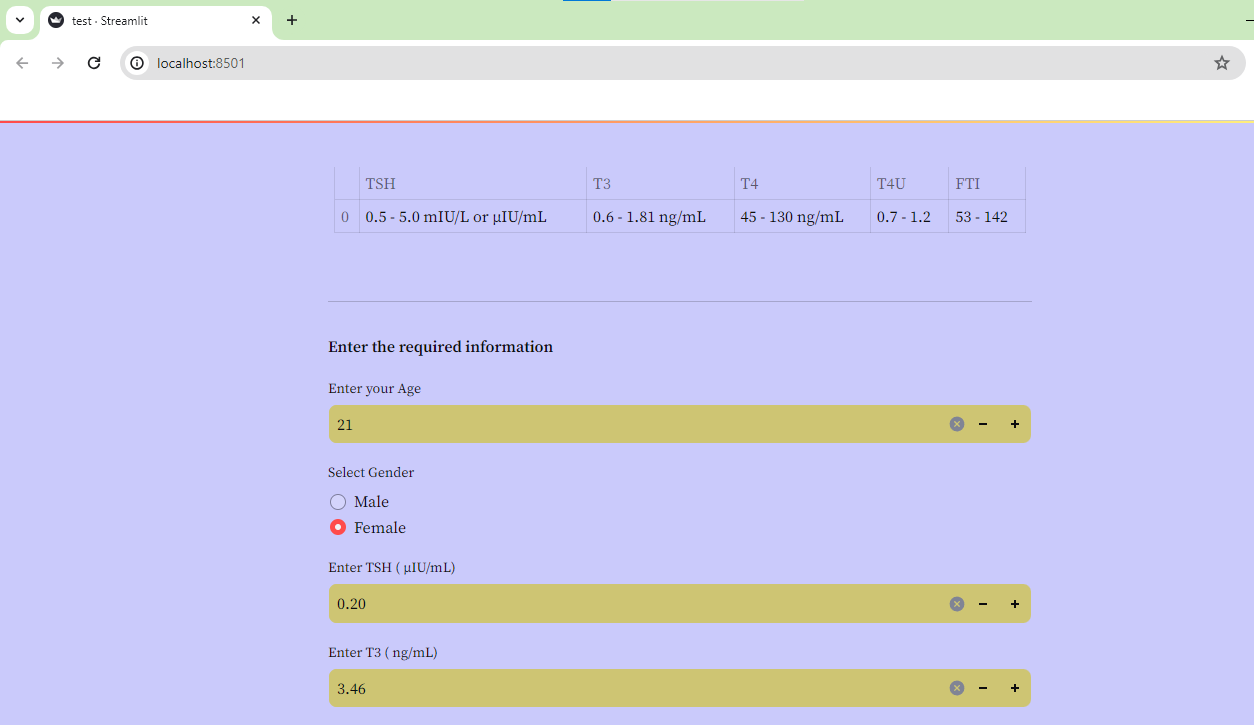
\includegraphics[scale=0.4]{result2.png}
\caption{Result 2}
\end{figure}

\begin{figure}[h]
\centering
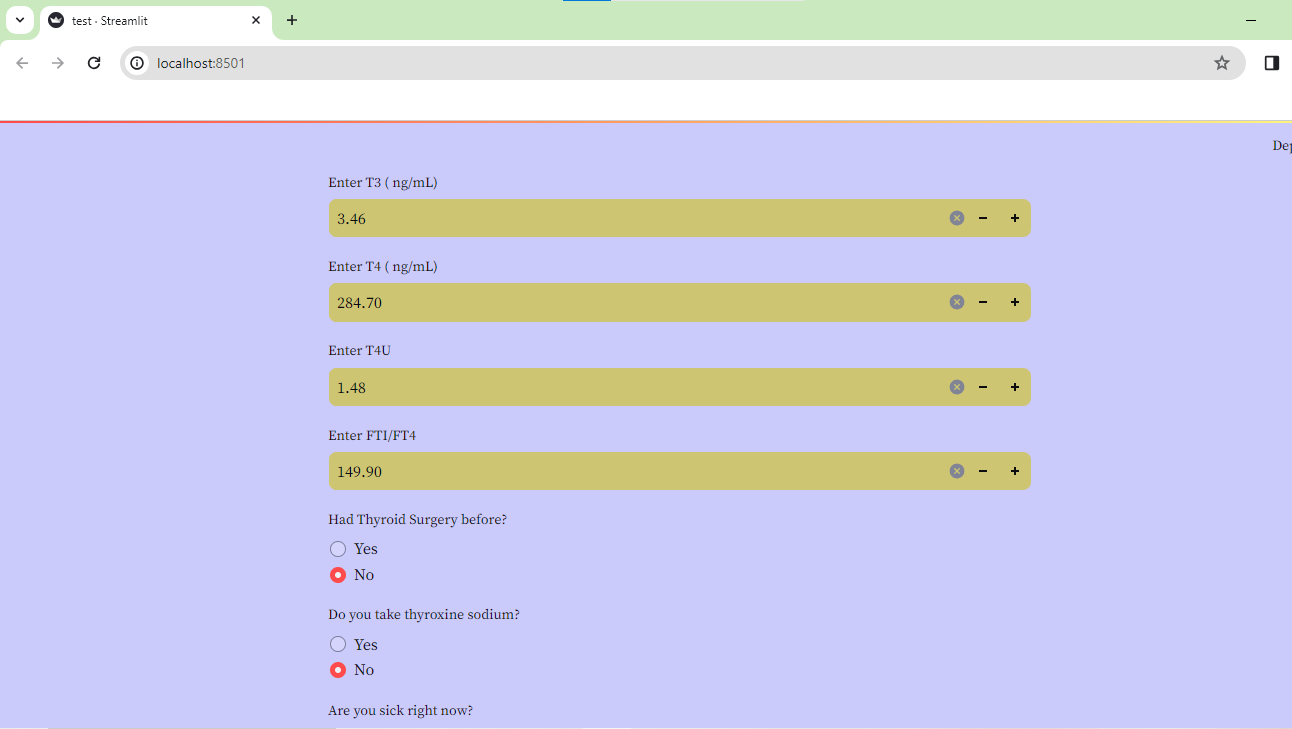
\includegraphics[scale=0.4]{result3.png}
\caption{Result 3}
\end{figure}

\begin{figure}[ht]
\centering
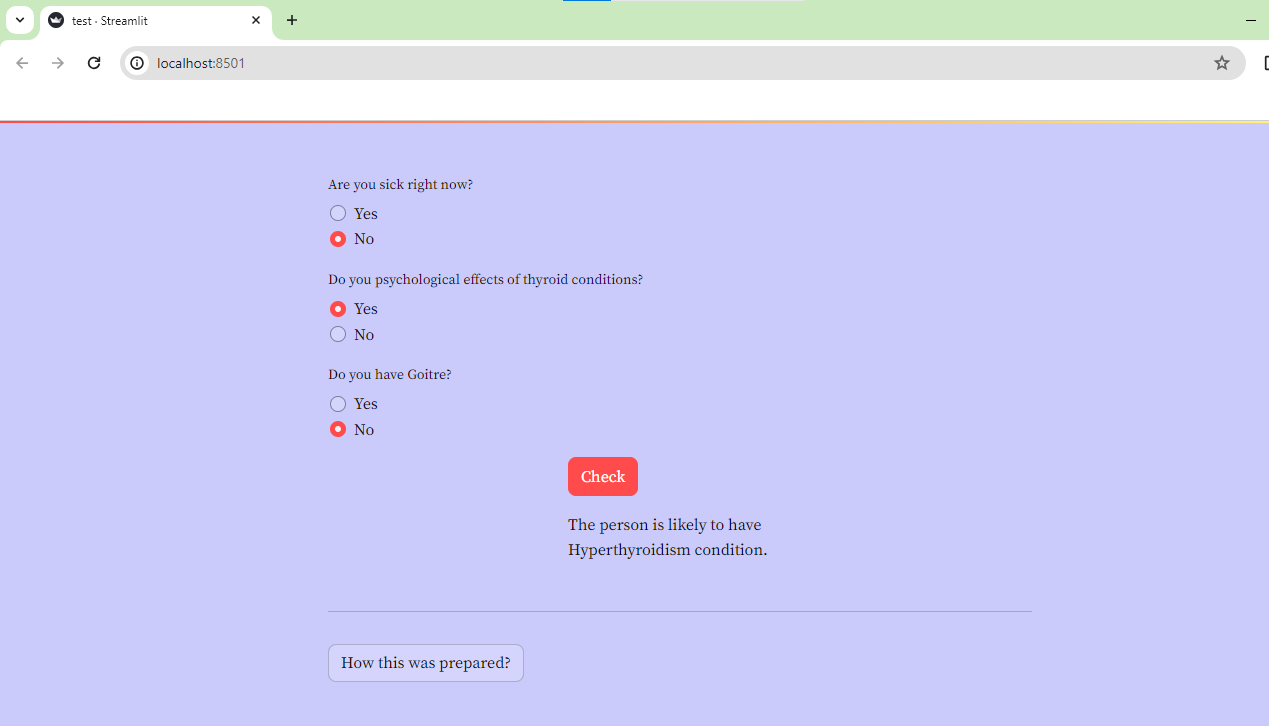
\includegraphics[scale=0.4]{result4.png}
\caption{Result 4}
\end{figure}
% \begin{figure}[ht]
%     \centering
%     \includegraphics[scale=0.2]{pictures/2.png}
%    % \caption{Gantt Chart}
%    % \label{fig:my_label}
% \end{figure}

% \begin{figure}[ht]
%     \centering
%     \includegraphics[scale=0.2]{pictures/3.png}
%    % \caption{Gantt Chart}
%    % \label{fig:my_label}
% \end{figure}

% \begin{figure}[ht]
%     \centering
%     \includegraphics[scale=0.2]{pictures/4.png}
%    % \caption{Gantt Chart}
%    % \label{fig:my_label}
% \end{figure}

% \begin{figure}[ht]
%     \centering
%     \includegraphics[scale=0.2]{pictures/5.png}
%    % \caption{Gantt Chart}
%    % \label{fig:my_label}
% \end{figure}
% \newpage
% \begin{figure}[ht]
%     \centering
%     \includegraphics[scale=0.2]{pictures/6.png}
%    % \caption{Gantt Chart}
%    % \label{fig:my_label}
% \end{figure}

% \begin{figure}[ht]
%     \centering
%     \includegraphics[scale=0.2]{pictures/7.png}
%    % \caption{Gantt Chart}
%    % \label{fig:my_label}
% \end{figure}

\nocite{goyal_2021}
\end{document}
